% Options for packages loaded elsewhere
% Options for packages loaded elsewhere
\PassOptionsToPackage{unicode}{hyperref}
\PassOptionsToPackage{hyphens}{url}
\PassOptionsToPackage{dvipsnames,svgnames,x11names}{xcolor}
%
\documentclass[
  letterpaper,
  DIV=11,
  numbers=noendperiod]{scrartcl}
\usepackage{xcolor}
\usepackage{amsmath,amssymb}
\setcounter{secnumdepth}{5}
\usepackage{iftex}
\ifPDFTeX
  \usepackage[T1]{fontenc}
  \usepackage[utf8]{inputenc}
  \usepackage{textcomp} % provide euro and other symbols
\else % if luatex or xetex
  \usepackage{unicode-math} % this also loads fontspec
  \defaultfontfeatures{Scale=MatchLowercase}
  \defaultfontfeatures[\rmfamily]{Ligatures=TeX,Scale=1}
\fi
\usepackage{lmodern}
\ifPDFTeX\else
  % xetex/luatex font selection
\fi
% Use upquote if available, for straight quotes in verbatim environments
\IfFileExists{upquote.sty}{\usepackage{upquote}}{}
\IfFileExists{microtype.sty}{% use microtype if available
  \usepackage[]{microtype}
  \UseMicrotypeSet[protrusion]{basicmath} % disable protrusion for tt fonts
}{}
\makeatletter
\@ifundefined{KOMAClassName}{% if non-KOMA class
  \IfFileExists{parskip.sty}{%
    \usepackage{parskip}
  }{% else
    \setlength{\parindent}{0pt}
    \setlength{\parskip}{6pt plus 2pt minus 1pt}}
}{% if KOMA class
  \KOMAoptions{parskip=half}}
\makeatother
% Make \paragraph and \subparagraph free-standing
\makeatletter
\ifx\paragraph\undefined\else
  \let\oldparagraph\paragraph
  \renewcommand{\paragraph}{
    \@ifstar
      \xxxParagraphStar
      \xxxParagraphNoStar
  }
  \newcommand{\xxxParagraphStar}[1]{\oldparagraph*{#1}\mbox{}}
  \newcommand{\xxxParagraphNoStar}[1]{\oldparagraph{#1}\mbox{}}
\fi
\ifx\subparagraph\undefined\else
  \let\oldsubparagraph\subparagraph
  \renewcommand{\subparagraph}{
    \@ifstar
      \xxxSubParagraphStar
      \xxxSubParagraphNoStar
  }
  \newcommand{\xxxSubParagraphStar}[1]{\oldsubparagraph*{#1}\mbox{}}
  \newcommand{\xxxSubParagraphNoStar}[1]{\oldsubparagraph{#1}\mbox{}}
\fi
\makeatother

\usepackage{color}
\usepackage{fancyvrb}
\newcommand{\VerbBar}{|}
\newcommand{\VERB}{\Verb[commandchars=\\\{\}]}
\DefineVerbatimEnvironment{Highlighting}{Verbatim}{commandchars=\\\{\}}
% Add ',fontsize=\small' for more characters per line
\usepackage{framed}
\definecolor{shadecolor}{RGB}{241,243,245}
\newenvironment{Shaded}{\begin{snugshade}}{\end{snugshade}}
\newcommand{\AlertTok}[1]{\textcolor[rgb]{0.68,0.00,0.00}{#1}}
\newcommand{\AnnotationTok}[1]{\textcolor[rgb]{0.37,0.37,0.37}{#1}}
\newcommand{\AttributeTok}[1]{\textcolor[rgb]{0.40,0.45,0.13}{#1}}
\newcommand{\BaseNTok}[1]{\textcolor[rgb]{0.68,0.00,0.00}{#1}}
\newcommand{\BuiltInTok}[1]{\textcolor[rgb]{0.00,0.23,0.31}{#1}}
\newcommand{\CharTok}[1]{\textcolor[rgb]{0.13,0.47,0.30}{#1}}
\newcommand{\CommentTok}[1]{\textcolor[rgb]{0.37,0.37,0.37}{#1}}
\newcommand{\CommentVarTok}[1]{\textcolor[rgb]{0.37,0.37,0.37}{\textit{#1}}}
\newcommand{\ConstantTok}[1]{\textcolor[rgb]{0.56,0.35,0.01}{#1}}
\newcommand{\ControlFlowTok}[1]{\textcolor[rgb]{0.00,0.23,0.31}{\textbf{#1}}}
\newcommand{\DataTypeTok}[1]{\textcolor[rgb]{0.68,0.00,0.00}{#1}}
\newcommand{\DecValTok}[1]{\textcolor[rgb]{0.68,0.00,0.00}{#1}}
\newcommand{\DocumentationTok}[1]{\textcolor[rgb]{0.37,0.37,0.37}{\textit{#1}}}
\newcommand{\ErrorTok}[1]{\textcolor[rgb]{0.68,0.00,0.00}{#1}}
\newcommand{\ExtensionTok}[1]{\textcolor[rgb]{0.00,0.23,0.31}{#1}}
\newcommand{\FloatTok}[1]{\textcolor[rgb]{0.68,0.00,0.00}{#1}}
\newcommand{\FunctionTok}[1]{\textcolor[rgb]{0.28,0.35,0.67}{#1}}
\newcommand{\ImportTok}[1]{\textcolor[rgb]{0.00,0.46,0.62}{#1}}
\newcommand{\InformationTok}[1]{\textcolor[rgb]{0.37,0.37,0.37}{#1}}
\newcommand{\KeywordTok}[1]{\textcolor[rgb]{0.00,0.23,0.31}{\textbf{#1}}}
\newcommand{\NormalTok}[1]{\textcolor[rgb]{0.00,0.23,0.31}{#1}}
\newcommand{\OperatorTok}[1]{\textcolor[rgb]{0.37,0.37,0.37}{#1}}
\newcommand{\OtherTok}[1]{\textcolor[rgb]{0.00,0.23,0.31}{#1}}
\newcommand{\PreprocessorTok}[1]{\textcolor[rgb]{0.68,0.00,0.00}{#1}}
\newcommand{\RegionMarkerTok}[1]{\textcolor[rgb]{0.00,0.23,0.31}{#1}}
\newcommand{\SpecialCharTok}[1]{\textcolor[rgb]{0.37,0.37,0.37}{#1}}
\newcommand{\SpecialStringTok}[1]{\textcolor[rgb]{0.13,0.47,0.30}{#1}}
\newcommand{\StringTok}[1]{\textcolor[rgb]{0.13,0.47,0.30}{#1}}
\newcommand{\VariableTok}[1]{\textcolor[rgb]{0.07,0.07,0.07}{#1}}
\newcommand{\VerbatimStringTok}[1]{\textcolor[rgb]{0.13,0.47,0.30}{#1}}
\newcommand{\WarningTok}[1]{\textcolor[rgb]{0.37,0.37,0.37}{\textit{#1}}}

\usepackage{longtable,booktabs,array}
\newcounter{none} % for unnumbered tables
\usepackage{calc} % for calculating minipage widths
% Correct order of tables after \paragraph or \subparagraph
\usepackage{etoolbox}
\makeatletter
\patchcmd\longtable{\par}{\if@noskipsec\mbox{}\fi\par}{}{}
\makeatother
% Allow footnotes in longtable head/foot
\IfFileExists{footnotehyper.sty}{\usepackage{footnotehyper}}{\usepackage{footnote}}
\makesavenoteenv{longtable}
\usepackage{graphicx}
\makeatletter
\newsavebox\pandoc@box
\newcommand*\pandocbounded[1]{% scales image to fit in text height/width
  \sbox\pandoc@box{#1}%
  \Gscale@div\@tempa{\textheight}{\dimexpr\ht\pandoc@box+\dp\pandoc@box\relax}%
  \Gscale@div\@tempb{\linewidth}{\wd\pandoc@box}%
  \ifdim\@tempb\p@<\@tempa\p@\let\@tempa\@tempb\fi% select the smaller of both
  \ifdim\@tempa\p@<\p@\scalebox{\@tempa}{\usebox\pandoc@box}%
  \else\usebox{\pandoc@box}%
  \fi%
}
% Set default figure placement to htbp
\def\fps@figure{htbp}
\makeatother





\setlength{\emergencystretch}{3em} % prevent overfull lines

\providecommand{\tightlist}{%
  \setlength{\itemsep}{0pt}\setlength{\parskip}{0pt}}



 


\usepackage{booktabs}
\usepackage{longtable}
\usepackage{array}
\usepackage{multirow}
\usepackage{wrapfig}
\usepackage{float}
\usepackage{colortbl}
\usepackage{pdflscape}
\usepackage{tabu}
\usepackage{threeparttable}
\usepackage{threeparttablex}
\usepackage[normalem]{ulem}
\usepackage{makecell}
\usepackage{xcolor}
\KOMAoption{captions}{tableheading}
\makeatletter
\@ifpackageloaded{caption}{}{\usepackage{caption}}
\AtBeginDocument{%
\ifdefined\contentsname
  \renewcommand*\contentsname{Table of contents}
\else
  \newcommand\contentsname{Table of contents}
\fi
\ifdefined\listfigurename
  \renewcommand*\listfigurename{List of Figures}
\else
  \newcommand\listfigurename{List of Figures}
\fi
\ifdefined\listtablename
  \renewcommand*\listtablename{List of Tables}
\else
  \newcommand\listtablename{List of Tables}
\fi
\ifdefined\figurename
  \renewcommand*\figurename{Figure}
\else
  \newcommand\figurename{Figure}
\fi
\ifdefined\tablename
  \renewcommand*\tablename{Table}
\else
  \newcommand\tablename{Table}
\fi
}
\@ifpackageloaded{float}{}{\usepackage{float}}
\floatstyle{ruled}
\@ifundefined{c@chapter}{\newfloat{codelisting}{h}{lop}}{\newfloat{codelisting}{h}{lop}[chapter]}
\floatname{codelisting}{Listing}
\newcommand*\listoflistings{\listof{codelisting}{List of Listings}}
\makeatother
\makeatletter
\makeatother
\makeatletter
\@ifpackageloaded{caption}{}{\usepackage{caption}}
\@ifpackageloaded{subcaption}{}{\usepackage{subcaption}}
\makeatother
\usepackage{bookmark}
\IfFileExists{xurl.sty}{\usepackage{xurl}}{} % add URL line breaks if available
\urlstyle{same}
\hypersetup{
  pdftitle={Les crèches favorisent-elles la natalité ? Une analyse départementale en France (2017--2023)},
  pdfauthor={Votre Nom},
  colorlinks=true,
  linkcolor={blue},
  filecolor={Maroon},
  citecolor={Blue},
  urlcolor={Blue},
  pdfcreator={LaTeX via pandoc}}


\title{Les crèches favorisent-elles la natalité ? Une analyse
départementale en France (2017--2023)}
\usepackage{etoolbox}
\makeatletter
\providecommand{\subtitle}[1]{% add subtitle to \maketitle
  \apptocmd{\@title}{\par {\large #1 \par}}{}{}
}
\makeatother
\subtitle{Introduction à l'Économétrie et à R}
\author{Votre Nom}
\date{2026-04-29}
\begin{document}
\maketitle

\renewcommand*\contentsname{Table of contents}
{
\setcounter{tocdepth}{3}
\tableofcontents
}

\section{Introduction}\label{introduction}

La France fait face à un déclin démographique inédit. Son taux de
natalité est passé de 12,6 naissances pour 1 000 habitants en 2010 à
environ 10,6 en 2017, puis à 9,9 en 2023. Le rapport annuel de l'INED
sur la conjoncture démographique (2025) enregistre pour la première fois
depuis un siècle une \textbf{croissance naturelle nulle dans
l'Hexagone}. Ce constat suscite un débat de politique publique croissant
autour des leviers susceptibles de soutenir la fécondité des ménages.

Parmi ces leviers, le développement des structures d'accueil du jeune
enfant (EAJE --- crèches, halte-garderies, micro-crèches) occupe une
place centrale dans les propositions récentes. L'intuition économique
est directe : des modes de garde accessibles réduisent le coût
d'opportunité de la maternité pour les femmes actives, facilitent la
conciliation entre vie professionnelle et parentalité, et devraient
ainsi encourager les naissances. Cette logique se retrouve dans
plusieurs recommandations institutionnelles : l'Académie nationale de
médecine place en deuxième position de ses préconisations la création de
100 000 places de crèches d'ici 2030 avec un financement pérenne de
l'État et des CAF. Dans la même veine, Elsa Hervy, déléguée générale de
la Fédération française des entreprises de crèches, défend cette
orientation dans un article de la revue \emph{Administration} (2025).

\subsection{Revue de littérature}\label{revue-de-littuxe9rature}

\textbf{À l'international}, la relation entre l'offre de garde formelle
et la fécondité est documentée dans de nombreux pays, avec des résultats
majoritairement positifs. Les études les plus robustes ont été conduites
en contexte nordique. Rindfuss, Guilkey et Morgan (2010) exploitent une
réforme d'ampleur en Norvège pour identifier une variation
\textbf{exogène} de l'offre de places et montrent un effet positif et
significatif sur la fécondité. Dans le même esprit, Mörk, Sjögren et
Svaleryd (2013) tirent parti d'une réforme suédoise sur le prix des
crèches pour établir un lien causal entre coût de la garde et décisions
de fécondité.

En Allemagne, Hener, Bauernschuster et Rainer (2013) mobilisent une
stratégie de \textbf{double différence} dans un contexte
particulièrement favorable à l'identification : l'ex-Allemagne de l'Est
était largement dépourvue de places en crèche jusqu'au début des années
2000, et la mise en œuvre des politiques d'expansion a varié fortement
d'un \emph{Kreis} à l'autre, créant une variation locale exploitable.
Leur étude confirme un effet positif de l'augmentation de l'offre sur la
natalité, avec une hétérogénéité marquée selon l'ampleur de l'expansion
locale.

Plus généralement, des résultats convergents ont été obtenus au Japon,
en Corée du Sud et en Espagne --- à l'exception notable d'un cas
espagnol où les crèches privées sont associées à une relation négative
avec la natalité, suggérant que les caractéristiques de l'offre (public
vs.~privé, tarification) importent autant que son volume. Luci-Greulich
et Thévenon (2013), dans une étude portant sur 18 pays de l'OCDE,
montrent que les services d'accueil pour les enfants de moins de trois
ans exercent un effet potentiellement plus important sur la fécondité
que les congés parentaux ou les transferts financiers à la naissance.

\textbf{En France}, ce lien n'a, à notre connaissance, pas encore fait
l'objet d'une estimation causale directe au niveau infranational, ce qui
explique que les rapports institutionnels cités plus haut n'appuient pas
leurs recommandations sur une étude empirique française. Une analyse de
l'INSEE (2020) a certes montré qu'accroître l'offre de places en crèche
avait peu d'effet sur l'emploi des mères, tout en réduisant le recours
aux autres modes de garde --- mais la question de l'effet sur la
natalité reste ouverte.

\subsection{Contribution de ce
travail}\label{contribution-de-ce-travail}

Ce travail propose une première approche empirique de cette question à
l'échelle des 96 départements métropolitains français, pour les années
\textbf{2017} et \textbf{2023}. En mobilisant les données CNAF sur les
taux de couverture petite enfance et les statistiques d'état civil de
l'INSEE, nous tentons d'évaluer si l'évolution de l'offre d'accueil est
associée à une évolution du taux de natalité. Si la méthode retenue ---
une approche en double différence --- est plus simple que les stratégies
d'identification exploitées dans les études nordiques ou allemandes, et
demeure exposée à certains problèmes d'endogénéité, elle constitue un
point de départ rigoureux pour documenter ce lien dans le contexte
français.

\begin{center}\rule{0.5\linewidth}{0.5pt}\end{center}

\section{Données}\label{donnuxe9es}

La base de données mobilisée dans cette étude est construite par
appariement de trois sources statistiques publiques portant sur les
\textbf{96 départements métropolitains} pour les années \textbf{2017} et
\textbf{2023} : les données de couverture petite enfance (CNAF), les
statistiques de naissances et de population (INSEE), et les données
d'emploi salarié départemental (INSEE). Les DROM-COM sont exclus : leurs
caractéristiques structurelles sont trop éloignées de celles des
départements métropolitains et leurs valeurs atypiques de natalité
biaiseraient les estimations.

Tous les identifiants géographiques sont harmonisés sous forme de chaîne
de caractères afin de traiter correctement les codes \texttt{2A} et
\texttt{2B} lors des fusions.

\begin{Shaded}
\begin{Highlighting}[]
\FunctionTok{library}\NormalTok{(readxl)}
\FunctionTok{library}\NormalTok{(dplyr)}
\FunctionTok{library}\NormalTok{(tidyr)}
\FunctionTok{library}\NormalTok{(stringr)}
\FunctionTok{library}\NormalTok{(knitr)}
\FunctionTok{library}\NormalTok{(kableExtra)}
\FunctionTok{library}\NormalTok{(ggplot2)}
\FunctionTok{library}\NormalTok{(psych)}
\FunctionTok{library}\NormalTok{(ggrepel)}

\CommentTok{\# Codes des 96 départements métropolitains}
\NormalTok{codes\_metro }\OtherTok{\textless{}{-}} \FunctionTok{c}\NormalTok{(}\FunctionTok{sprintf}\NormalTok{(}\StringTok{"\%02d"}\NormalTok{, }\DecValTok{1}\SpecialCharTok{:}\DecValTok{19}\NormalTok{), }\StringTok{"2A"}\NormalTok{, }\StringTok{"2B"}\NormalTok{, }\FunctionTok{as.character}\NormalTok{(}\DecValTok{21}\SpecialCharTok{:}\DecValTok{95}\NormalTok{))}
\end{Highlighting}
\end{Shaded}

\subsection{Taux de couverture petite enfance
(CNAF)}\label{taux-de-couverture-petite-enfance-cnaf}

Les données de couverture sont issues de deux fichiers de la CNAF :
\texttt{txcouv\_pe\_dep\_hist.csv} pour les années antérieures à 2022
(qui contient donc 2017), et \texttt{txcouv\_pe\_dep.csv} pour
2022-2023. Chacun est filtré sur les départements métropolitains, puis
les années 2017 et 2023 sont extraites séparément.

\begin{Shaded}
\begin{Highlighting}[]
\CommentTok{\# Chargement et filtrage sur la métropole}
\NormalTok{crechedep2223 }\OtherTok{\textless{}{-}} \FunctionTok{read.csv}\NormalTok{(}\StringTok{"txcouv\_pe\_dep.csv"}\NormalTok{,      }\AttributeTok{sep =} \StringTok{";"}\NormalTok{) }\SpecialCharTok{|\textgreater{}}
  \FunctionTok{filter}\NormalTok{(Numéro.Département }\SpecialCharTok{\%in\%}\NormalTok{ codes\_metro)}

\NormalTok{crechedep1722 }\OtherTok{\textless{}{-}} \FunctionTok{read.csv}\NormalTok{(}\StringTok{"txcouv\_pe\_dep\_hist.csv"}\NormalTok{, }\AttributeTok{sep =} \StringTok{";"}\NormalTok{) }\SpecialCharTok{|\textgreater{}}
  \FunctionTok{filter}\NormalTok{(Numéro.Département }\SpecialCharTok{\%in\%}\NormalTok{ codes\_metro)}

\CommentTok{\# Extraction des années cibles et sélection des variables utiles}
\NormalTok{vars\_couv }\OtherTok{\textless{}{-}} \FunctionTok{c}\NormalTok{(}\StringTok{"Date.référence"}\NormalTok{, }\StringTok{"Numéro.Département"}\NormalTok{, }\StringTok{"Nom.Département"}\NormalTok{,}
               \StringTok{"Taux.de.couv.EAJE.PSU"}\NormalTok{, }\StringTok{"Taux.de.couv.hors.EAJE.PSU"}\NormalTok{,}
               \StringTok{"Taux.de.couv.EAJE...ensemble"}\NormalTok{, }\StringTok{"Taux.de.couv.préscolarisation"}\NormalTok{,}
               \StringTok{"Taux.de.couv.assistante.maternelle"}\NormalTok{, }\StringTok{"Taux.de.couv.salariée.à.domicile"}\NormalTok{,}
               \StringTok{"Taux.de.couv.accueil.individuel...ensemble"}\NormalTok{, }\StringTok{"Taux.de.couv.global"}\NormalTok{)}

\NormalTok{noms\_couv }\OtherTok{\textless{}{-}} \FunctionTok{c}\NormalTok{(}\StringTok{"année"}\NormalTok{, }\StringTok{"Code.de.département"}\NormalTok{, }\StringTok{"département"}\NormalTok{,}
               \StringTok{"Taux.de.couv.EAJE.PSU"}\NormalTok{, }\StringTok{"Taux.de.couv.hors.EAJE.PSU"}\NormalTok{,}
               \StringTok{"Taux.de.couv.EAJE...ensemble"}\NormalTok{, }\StringTok{"Taux.de.couv.préscolarisation"}\NormalTok{,}
               \StringTok{"Taux.de.couv.assistante.maternelle"}\NormalTok{, }\StringTok{"Taux.de.couv.salariée.à.domicile"}\NormalTok{,}
               \StringTok{"Taux.de.couv.accueil.individuel...ensemble"}\NormalTok{, }\StringTok{"Taux.de.couv.global"}\NormalTok{)}

\NormalTok{crechedep17 }\OtherTok{\textless{}{-}}\NormalTok{ crechedep1722 }\SpecialCharTok{|\textgreater{}} \FunctionTok{filter}\NormalTok{(Date.référence }\SpecialCharTok{==} \DecValTok{2017}\NormalTok{) }\SpecialCharTok{|\textgreater{}}
  \FunctionTok{select}\NormalTok{(}\FunctionTok{all\_of}\NormalTok{(vars\_couv)) }\SpecialCharTok{|\textgreater{}} \FunctionTok{setNames}\NormalTok{(noms\_couv)}

\NormalTok{crechedep23 }\OtherTok{\textless{}{-}}\NormalTok{ crechedep2223 }\SpecialCharTok{|\textgreater{}} \FunctionTok{filter}\NormalTok{(Date.référence }\SpecialCharTok{==} \DecValTok{2023}\NormalTok{) }\SpecialCharTok{|\textgreater{}}
  \FunctionTok{select}\NormalTok{(}\FunctionTok{all\_of}\NormalTok{(vars\_couv)) }\SpecialCharTok{|\textgreater{}} \FunctionTok{setNames}\NormalTok{(noms\_couv)}
\end{Highlighting}
\end{Shaded}

Le \textbf{taux de couverture} mesure la capacité d'accueil théorique
pour 100 enfants de moins de 3 ans dans un département. Il se décompose
en plusieurs modes d'accueil :

{\def\LTcaptype{none} % do not increment counter
\begin{longtable}[]{@{}
  >{\raggedright\arraybackslash}p{(\linewidth - 4\tabcolsep) * \real{0.3333}}
  >{\raggedright\arraybackslash}p{(\linewidth - 4\tabcolsep) * \real{0.3333}}
  >{\raggedright\arraybackslash}p{(\linewidth - 4\tabcolsep) * \real{0.3333}}@{}}
\toprule\noalign{}
\begin{minipage}[b]{\linewidth}\raggedright
Mode
\end{minipage} & \begin{minipage}[b]{\linewidth}\raggedright
Variable
\end{minipage} & \begin{minipage}[b]{\linewidth}\raggedright
Nature
\end{minipage} \\
\midrule\noalign{}
\endhead
\bottomrule\noalign{}
\endlastfoot
EAJE PSU & \texttt{Taux.de.couv.EAJE.PSU} & Crèches collectives,
halte-garderies (financement CAF-PSU) \\
Hors PSU & \texttt{Taux.de.couv.hors.EAJE.PSU} & Micro-crèches PAJE \\
Préscolarisation & \texttt{Taux.de.couv.préscolarisation} & Enfants
\textless{} 3 ans en maternelle \\
Assistante maternelle & \texttt{Taux.de.couv.assistante.maternelle} &
Accueil individuel agréé \\
Salariée à domicile & \texttt{Taux.de.couv.salariée.à.domicile} & Garde
au domicile \\
\textbf{Global} & \texttt{Taux.de.couv.global} & Agrégat de tous les
modes \\
\end{longtable}
}

Pour l'estimation, on construit deux variables synthétiques selon la
nature de l'accueil. L'accueil \textbf{collectif} regroupe les
structures relevant principalement de décisions publiques
d'investissement ; l'accueil \textbf{individuel} dépend davantage du
marché local et des préférences des familles. Cette distinction permet
de tester si l'effet sur la natalité diffère selon le type de garde.

\[\text{Couverture collective} = \text{EAJE PSU} + \text{Hors EAJE PSU} + \text{Préscolarisation}\]
\[\text{Couverture individuelle} = \text{Assistante maternelle} + \text{Salariée à domicile}\]

Les virgules décimales présentes dans les fichiers bruts CNAF sont
remplacées par des points (\texttt{gsub(",",\ ".",\ .)}) avant toute
conversion numérique.

\begin{Shaded}
\begin{Highlighting}[]
\CommentTok{\# Conversion numérique et construction des agrégats collectif / individuel}
\NormalTok{construire\_taux\_couv }\OtherTok{\textless{}{-}} \ControlFlowTok{function}\NormalTok{(df) \{}
\NormalTok{  df }\SpecialCharTok{|\textgreater{}}
    \FunctionTok{mutate}\NormalTok{(}
\NormalTok{      Code.de.département }\OtherTok{=} \FunctionTok{as.character}\NormalTok{(Code.de.département),}
      \FunctionTok{across}\NormalTok{(}\FunctionTok{starts\_with}\NormalTok{(}\StringTok{"Taux"}\NormalTok{), }\SpecialCharTok{\textasciitilde{}} \FunctionTok{as.numeric}\NormalTok{(}\FunctionTok{gsub}\NormalTok{(}\StringTok{","}\NormalTok{, }\StringTok{"."}\NormalTok{, .))),}
      \AttributeTok{Taux.de.couv.collectif  =}\NormalTok{ Taux.de.couv.EAJE.PSU }\SpecialCharTok{+}
\NormalTok{                                 Taux.de.couv.hors.EAJE.PSU }\SpecialCharTok{+}
\NormalTok{                                 Taux.de.couv.préscolarisation,}
      \AttributeTok{Taux.de.couv.individuel =}\NormalTok{ Taux.de.couv.assistante.maternelle }\SpecialCharTok{+}
\NormalTok{                                 Taux.de.couv.salariée.à.domicile}
\NormalTok{    )}
\NormalTok{\}}

\NormalTok{crechedep17 }\OtherTok{\textless{}{-}} \FunctionTok{construire\_taux\_couv}\NormalTok{(crechedep17)}
\NormalTok{crechedep23 }\OtherTok{\textless{}{-}} \FunctionTok{construire\_taux\_couv}\NormalTok{(crechedep23)}
\end{Highlighting}
\end{Shaded}

\subsection{Taux de natalité (INSEE)}\label{taux-de-natalituxe9-insee}

Les données de naissances sont issues du tableau N1D de l'INSEE (état
civil). Après suppression des lignes d'en-tête, les naissances sont
appariées aux populations départementales issues du recensement. Un
tableau de correspondance (\texttt{codes\_dep}) permet d'associer le nom
de département tel que fourni par l'INSEE au code officiel.

\begin{Shaded}
\begin{Highlighting}[]
\CommentTok{\# Table de correspondance nom → code département}
\NormalTok{codes\_dep }\OtherTok{\textless{}{-}} \FunctionTok{data.frame}\NormalTok{(}
\NormalTok{  Code.de.département }\OtherTok{=} \FunctionTok{c}\NormalTok{(}
    \StringTok{"01"}\NormalTok{,}\StringTok{"02"}\NormalTok{,}\StringTok{"03"}\NormalTok{,}\StringTok{"04"}\NormalTok{,}\StringTok{"05"}\NormalTok{,}\StringTok{"06"}\NormalTok{,}\StringTok{"07"}\NormalTok{,}\StringTok{"08"}\NormalTok{,}\StringTok{"09"}\NormalTok{,}\StringTok{"10"}\NormalTok{,}\StringTok{"11"}\NormalTok{,}\StringTok{"12"}\NormalTok{,}\StringTok{"13"}\NormalTok{,}\StringTok{"14"}\NormalTok{,}\StringTok{"15"}\NormalTok{,}
    \StringTok{"16"}\NormalTok{,}\StringTok{"17"}\NormalTok{,}\StringTok{"18"}\NormalTok{,}\StringTok{"19"}\NormalTok{,}\StringTok{"21"}\NormalTok{,}\StringTok{"22"}\NormalTok{,}\StringTok{"23"}\NormalTok{,}\StringTok{"24"}\NormalTok{,}\StringTok{"25"}\NormalTok{,}\StringTok{"26"}\NormalTok{,}\StringTok{"27"}\NormalTok{,}\StringTok{"28"}\NormalTok{,}\StringTok{"29"}\NormalTok{,}\StringTok{"2A"}\NormalTok{,}\StringTok{"2B"}\NormalTok{,}
    \StringTok{"30"}\NormalTok{,}\StringTok{"31"}\NormalTok{,}\StringTok{"32"}\NormalTok{,}\StringTok{"33"}\NormalTok{,}\StringTok{"34"}\NormalTok{,}\StringTok{"35"}\NormalTok{,}\StringTok{"36"}\NormalTok{,}\StringTok{"37"}\NormalTok{,}\StringTok{"38"}\NormalTok{,}\StringTok{"39"}\NormalTok{,}\StringTok{"40"}\NormalTok{,}\StringTok{"41"}\NormalTok{,}\StringTok{"42"}\NormalTok{,}\StringTok{"43"}\NormalTok{,}\StringTok{"44"}\NormalTok{,}
    \StringTok{"45"}\NormalTok{,}\StringTok{"46"}\NormalTok{,}\StringTok{"47"}\NormalTok{,}\StringTok{"48"}\NormalTok{,}\StringTok{"49"}\NormalTok{,}\StringTok{"50"}\NormalTok{,}\StringTok{"51"}\NormalTok{,}\StringTok{"52"}\NormalTok{,}\StringTok{"53"}\NormalTok{,}\StringTok{"54"}\NormalTok{,}\StringTok{"55"}\NormalTok{,}\StringTok{"56"}\NormalTok{,}\StringTok{"57"}\NormalTok{,}\StringTok{"58"}\NormalTok{,}\StringTok{"59"}\NormalTok{,}
    \StringTok{"60"}\NormalTok{,}\StringTok{"61"}\NormalTok{,}\StringTok{"62"}\NormalTok{,}\StringTok{"63"}\NormalTok{,}\StringTok{"64"}\NormalTok{,}\StringTok{"65"}\NormalTok{,}\StringTok{"66"}\NormalTok{,}\StringTok{"67"}\NormalTok{,}\StringTok{"68"}\NormalTok{,}\StringTok{"69"}\NormalTok{,}\StringTok{"70"}\NormalTok{,}\StringTok{"71"}\NormalTok{,}\StringTok{"72"}\NormalTok{,}\StringTok{"73"}\NormalTok{,}\StringTok{"74"}\NormalTok{,}
    \StringTok{"75"}\NormalTok{,}\StringTok{"76"}\NormalTok{,}\StringTok{"77"}\NormalTok{,}\StringTok{"78"}\NormalTok{,}\StringTok{"79"}\NormalTok{,}\StringTok{"80"}\NormalTok{,}\StringTok{"81"}\NormalTok{,}\StringTok{"82"}\NormalTok{,}\StringTok{"83"}\NormalTok{,}\StringTok{"84"}\NormalTok{,}\StringTok{"85"}\NormalTok{,}\StringTok{"86"}\NormalTok{,}\StringTok{"87"}\NormalTok{,}\StringTok{"88"}\NormalTok{,}\StringTok{"89"}\NormalTok{,}
    \StringTok{"90"}\NormalTok{,}\StringTok{"91"}\NormalTok{,}\StringTok{"92"}\NormalTok{,}\StringTok{"93"}\NormalTok{,}\StringTok{"94"}\NormalTok{,}\StringTok{"95"}\NormalTok{),}
\NormalTok{  département }\OtherTok{=} \FunctionTok{c}\NormalTok{(}
    \StringTok{"Ain"}\NormalTok{,}\StringTok{"Aisne"}\NormalTok{,}\StringTok{"Allier"}\NormalTok{,}\StringTok{"Alpes{-}de{-}Haute{-}Provence"}\NormalTok{,}\StringTok{"Hautes{-}Alpes"}\NormalTok{,}
    \StringTok{"Alpes{-}Maritimes"}\NormalTok{,}\StringTok{"Ardèche"}\NormalTok{,}\StringTok{"Ardennes"}\NormalTok{,}\StringTok{"Ariège"}\NormalTok{,}\StringTok{"Aube"}\NormalTok{,}\StringTok{"Aude"}\NormalTok{,}\StringTok{"Aveyron"}\NormalTok{,}
    \StringTok{"Bouches{-}du{-}Rhône"}\NormalTok{,}\StringTok{"Calvados"}\NormalTok{,}\StringTok{"Cantal"}\NormalTok{,}\StringTok{"Charente"}\NormalTok{,}\StringTok{"Charente{-}Maritime"}\NormalTok{,}\StringTok{"Cher"}\NormalTok{,}
    \StringTok{"Corrèze"}\NormalTok{,}\StringTok{"Côte{-}d\textquotesingle{}Or"}\NormalTok{,}\StringTok{"Côtes{-}d\textquotesingle{}Armor"}\NormalTok{,}\StringTok{"Creuse"}\NormalTok{,}\StringTok{"Dordogne"}\NormalTok{,}\StringTok{"Doubs"}\NormalTok{,}\StringTok{"Drôme"}\NormalTok{,}
    \StringTok{"Eure"}\NormalTok{,}\StringTok{"Eure{-}et{-}Loir"}\NormalTok{,}\StringTok{"Finistère"}\NormalTok{,}\StringTok{"Corse{-}du{-}Sud"}\NormalTok{,}\StringTok{"Haute{-}Corse"}\NormalTok{,}\StringTok{"Gard"}\NormalTok{,}
    \StringTok{"Haute{-}Garonne"}\NormalTok{,}\StringTok{"Gers"}\NormalTok{,}\StringTok{"Gironde"}\NormalTok{,}\StringTok{"Hérault"}\NormalTok{,}\StringTok{"Ille{-}et{-}Vilaine"}\NormalTok{,}\StringTok{"Indre"}\NormalTok{,}
    \StringTok{"Indre{-}et{-}Loire"}\NormalTok{,}\StringTok{"Isère"}\NormalTok{,}\StringTok{"Jura"}\NormalTok{,}\StringTok{"Landes"}\NormalTok{,}\StringTok{"Loir{-}et{-}Cher"}\NormalTok{,}\StringTok{"Loire"}\NormalTok{,}
    \StringTok{"Haute{-}Loire"}\NormalTok{,}\StringTok{"Loire{-}Atlantique"}\NormalTok{,}\StringTok{"Loiret"}\NormalTok{,}\StringTok{"Lot"}\NormalTok{,}\StringTok{"Lot{-}et{-}Garonne"}\NormalTok{,}\StringTok{"Lozère"}\NormalTok{,}
    \StringTok{"Maine{-}et{-}Loire"}\NormalTok{,}\StringTok{"Manche"}\NormalTok{,}\StringTok{"Marne"}\NormalTok{,}\StringTok{"Haute{-}Marne"}\NormalTok{,}\StringTok{"Mayenne"}\NormalTok{,}
    \StringTok{"Meurthe{-}et{-}Moselle"}\NormalTok{,}\StringTok{"Meuse"}\NormalTok{,}\StringTok{"Morbihan"}\NormalTok{,}\StringTok{"Moselle"}\NormalTok{,}\StringTok{"Nièvre"}\NormalTok{,}\StringTok{"Nord"}\NormalTok{,}\StringTok{"Oise"}\NormalTok{,}
    \StringTok{"Orne"}\NormalTok{,}\StringTok{"Pas{-}de{-}Calais"}\NormalTok{,}\StringTok{"Puy{-}de{-}Dôme"}\NormalTok{,}\StringTok{"Pyrénées{-}Atlantiques"}\NormalTok{,}
    \StringTok{"Hautes{-}Pyrénées"}\NormalTok{,}\StringTok{"Pyrénées{-}Orientales"}\NormalTok{,}\StringTok{"Bas{-}Rhin"}\NormalTok{,}\StringTok{"Haut{-}Rhin"}\NormalTok{,}\StringTok{"Rhône"}\NormalTok{,}
    \StringTok{"Haute{-}Saône"}\NormalTok{,}\StringTok{"Saône{-}et{-}Loire"}\NormalTok{,}\StringTok{"Sarthe"}\NormalTok{,}\StringTok{"Savoie"}\NormalTok{,}\StringTok{"Haute{-}Savoie"}\NormalTok{,}\StringTok{"Paris"}\NormalTok{,}
    \StringTok{"Seine{-}Maritime"}\NormalTok{,}\StringTok{"Seine{-}et{-}Marne"}\NormalTok{,}\StringTok{"Yvelines"}\NormalTok{,}\StringTok{"Deux{-}Sèvres"}\NormalTok{,}\StringTok{"Somme"}\NormalTok{,}\StringTok{"Tarn"}\NormalTok{,}
    \StringTok{"Tarn{-}et{-}Garonne"}\NormalTok{,}\StringTok{"Var"}\NormalTok{,}\StringTok{"Vaucluse"}\NormalTok{,}\StringTok{"Vendée"}\NormalTok{,}\StringTok{"Vienne"}\NormalTok{,}\StringTok{"Haute{-}Vienne"}\NormalTok{,}
    \StringTok{"Vosges"}\NormalTok{,}\StringTok{"Yonne"}\NormalTok{,}\StringTok{"Territoire de Belfort"}\NormalTok{,}\StringTok{"Essonne"}\NormalTok{,}\StringTok{"Hauts{-}de{-}Seine"}\NormalTok{,}
    \StringTok{"Seine{-}Saint{-}Denis"}\NormalTok{,}\StringTok{"Val{-}de{-}Marne"}\NormalTok{,}\StringTok{"Val{-}d\textquotesingle{}Oise"}\NormalTok{)}
\NormalTok{)}

\CommentTok{\# Chargement, nettoyage et appariement des naissances}
\NormalTok{charger\_naissances }\OtherTok{\textless{}{-}} \ControlFlowTok{function}\NormalTok{(fichier, }\AttributeTok{ext =} \StringTok{"xlsx"}\NormalTok{) \{}
\NormalTok{  lire }\OtherTok{\textless{}{-}} \ControlFlowTok{if}\NormalTok{ (ext }\SpecialCharTok{==} \StringTok{"xls"}\NormalTok{) read\_xls }\ControlFlowTok{else}\NormalTok{ read\_xlsx}
  \FunctionTok{lire}\NormalTok{(fichier) }\SpecialCharTok{|\textgreater{}}
    \FunctionTok{slice}\NormalTok{(}\SpecialCharTok{{-}}\NormalTok{(}\DecValTok{1}\SpecialCharTok{:}\DecValTok{3}\NormalTok{)) }\SpecialCharTok{|\textgreater{}}
    \FunctionTok{select}\NormalTok{(}\DecValTok{1}\SpecialCharTok{:}\DecValTok{2}\NormalTok{) }\SpecialCharTok{|\textgreater{}}
    \FunctionTok{setNames}\NormalTok{(}\FunctionTok{c}\NormalTok{(}\StringTok{"département"}\NormalTok{, }\StringTok{"naissances"}\NormalTok{)) }\SpecialCharTok{|\textgreater{}}
    \FunctionTok{merge}\NormalTok{(codes\_dep, }\AttributeTok{by =} \StringTok{"département"}\NormalTok{, }\AttributeTok{all.x =} \ConstantTok{TRUE}\NormalTok{) }\SpecialCharTok{|\textgreater{}}
    \FunctionTok{filter}\NormalTok{(}\SpecialCharTok{!}\FunctionTok{is.na}\NormalTok{(Code.de.département),}
\NormalTok{           Code.de.département }\SpecialCharTok{\%in\%}\NormalTok{ codes\_metro)}
\NormalTok{\}}

\NormalTok{tauxdenatalite17 }\OtherTok{\textless{}{-}} \FunctionTok{charger\_naissances}\NormalTok{(}\StringTok{"N1D.xls"}\NormalTok{,  }\AttributeTok{ext =} \StringTok{"xls"}\NormalTok{)}
\NormalTok{tauxdenatalite23 }\OtherTok{\textless{}{-}} \FunctionTok{charger\_naissances}\NormalTok{(}\StringTok{"irsocsd2023\_dd9\_xlsx/n1d.xlsx"}\NormalTok{, }\AttributeTok{ext =} \StringTok{"xlsx"}\NormalTok{)}
\end{Highlighting}
\end{Shaded}

Les populations départementales sont extraites des fichiers de
recensement (onglet ``Départements''). Seules les colonnes
d'identification et d'effectif total sont conservées ; les colonnes
intermédiaires sont supprimées.

\begin{Shaded}
\begin{Highlighting}[]
\NormalTok{charger\_population }\OtherTok{\textless{}{-}} \ControlFlowTok{function}\NormalTok{(fichier, }\AttributeTok{ext =} \StringTok{"xlsx"}\NormalTok{) \{}
\NormalTok{  lire }\OtherTok{\textless{}{-}} \ControlFlowTok{if}\NormalTok{ (ext }\SpecialCharTok{==} \StringTok{"xls"}\NormalTok{) read\_xls }\ControlFlowTok{else}\NormalTok{ read\_xlsx}
  \FunctionTok{lire}\NormalTok{(fichier, }\AttributeTok{sheet =} \StringTok{"Départements"}\NormalTok{) }\SpecialCharTok{|\textgreater{}}
    \FunctionTok{setNames}\NormalTok{(}\FunctionTok{c}\NormalTok{(}\StringTok{"a"}\NormalTok{,}\StringTok{"b"}\NormalTok{,}\StringTok{"Code.de.département"}\NormalTok{,}\StringTok{"département"}\NormalTok{,}\StringTok{"d"}\NormalTok{,}\StringTok{"e"}\NormalTok{,}\StringTok{"f"}\NormalTok{,}\StringTok{"g"}\NormalTok{,}\StringTok{"population"}\NormalTok{)) }\SpecialCharTok{|\textgreater{}}
    \FunctionTok{select}\NormalTok{(Code.de.département, département, population) }\SpecialCharTok{|\textgreater{}}
    \FunctionTok{slice}\NormalTok{(}\SpecialCharTok{{-}}\NormalTok{(}\DecValTok{1}\SpecialCharTok{:}\DecValTok{7}\NormalTok{)) }\SpecialCharTok{|\textgreater{}}
    \FunctionTok{filter}\NormalTok{(Code.de.département }\SpecialCharTok{\%in\%}\NormalTok{ codes\_metro)}
\NormalTok{\}}

\NormalTok{population17 }\OtherTok{\textless{}{-}} \FunctionTok{charger\_population}\NormalTok{(}\StringTok{"ensemble.xls"}\NormalTok{, }\AttributeTok{ext =} \StringTok{"xls"}\NormalTok{)}
\NormalTok{population23 }\OtherTok{\textless{}{-}} \FunctionTok{charger\_population}\NormalTok{(}\StringTok{"ensemble.xlsx"}\NormalTok{, }\AttributeTok{ext =} \StringTok{"xlsx"}\NormalTok{)}
\end{Highlighting}
\end{Shaded}

Le taux de natalité est ensuite calculé selon la formule :

\[\text{Taux de natalité}_{d,t} = \frac{\text{Naissances}_{d,t}}{\text{Population}_{d,t}} \times 1000\]

Les espaces insécables utilisés comme séparateurs de milliers dans les
fichiers bruts sont supprimés avec \texttt{gsub} avant conversion
numérique.

\begin{Shaded}
\begin{Highlighting}[]
\NormalTok{calculer\_taux\_nat }\OtherTok{\textless{}{-}} \ControlFlowTok{function}\NormalTok{(naissances\_df, population\_df, nom\_var) \{}
  \FunctionTok{merge}\NormalTok{(naissances\_df, population\_df, }\AttributeTok{by =} \StringTok{"Code.de.département"}\NormalTok{) }\SpecialCharTok{|\textgreater{}}
    \FunctionTok{mutate}\NormalTok{(}
      \AttributeTok{naissances =} \FunctionTok{as.numeric}\NormalTok{(}\FunctionTok{gsub}\NormalTok{(}\StringTok{"[ ,]"}\NormalTok{, }\StringTok{""}\NormalTok{, naissances)),}
      \AttributeTok{population =} \FunctionTok{as.numeric}\NormalTok{(}\FunctionTok{gsub}\NormalTok{(}\StringTok{"[ ,]"}\NormalTok{, }\StringTok{""}\NormalTok{, population)),}
      \SpecialCharTok{!!}\AttributeTok{nom\_var  :=}\NormalTok{ (naissances }\SpecialCharTok{/}\NormalTok{ population) }\SpecialCharTok{*} \DecValTok{1000}\NormalTok{,}
\NormalTok{      Code.de.département }\OtherTok{=} \FunctionTok{as.character}\NormalTok{(Code.de.département)}
\NormalTok{    ) }\SpecialCharTok{|\textgreater{}}
    \FunctionTok{select}\NormalTok{(Code.de.département, naissances, population, }\SpecialCharTok{!!}\FunctionTok{sym}\NormalTok{(nom\_var))}
\NormalTok{\}}

\NormalTok{taux17 }\OtherTok{\textless{}{-}} \FunctionTok{calculer\_taux\_nat}\NormalTok{(tauxdenatalite17, population17, }\StringTok{"taux\_natalite\_2017"}\NormalTok{)}
\NormalTok{taux23 }\OtherTok{\textless{}{-}} \FunctionTok{calculer\_taux\_nat}\NormalTok{(tauxdenatalite23, population23, }\StringTok{"taux\_natalite\_2023"}\NormalTok{)}
\end{Highlighting}
\end{Shaded}

On peut vérifier la plausibilité des valeurs : le taux moyen sur les 96
départements métropolitains est de \textbf{9.93 ‰} en 2017 et
\textbf{8.58 ‰} en 2023, cohérents avec les taux nationaux publiés par
l'INSEE (qui incluent également les DROM, légèrement plus élevés).

\subsection{Indice d'emploi relatif
(INSEE)}\label{indice-demploi-relatif-insee}

Les données d'emploi salarié sont issues du tableau longitudinal T201 de
l'INSEE. Après suppression des lignes d'en-tête et filtrage des entités
non départementales, seules les colonnes 2017 et 2023 sont conservées.

Le marché du travail local est une variable confondante incontournable :
un département économiquement dynamique attire des actifs en âge de
procréer, ce qui peut simultanément accroître la demande de crèches et
le taux de natalité. Omettre cette variable conduirait à surestimer
l'effet propre des crèches.

On construit un \textbf{indice d'emploi relatif} en normalisant le taux
d'emploi brut de chaque département par le taux d'emploi national :

\[\text{Indice d'emploi}_{d,t} = \frac{\text{Emplois}_{d,t} / \text{Population}_{d,t}}{\displaystyle\sum_d \text{Emplois}_{d,t} \big/ \sum_d \text{Population}_{d,t}} \times 100\]

Un indice de 100 correspond à la moyenne nationale. Les valeurs
supérieures à 100 indiquent une densité d'emploi supérieure à la moyenne
(Paris, Hauts-de-Seine) ; inférieures à 100, une économie locale moins
dense (départements ruraux).

\begin{Shaded}
\begin{Highlighting}[]
\NormalTok{emploi\_raw }\OtherTok{\textless{}{-}} \FunctionTok{read\_xlsx}\NormalTok{(}\StringTok{"t201.xlsx"}\NormalTok{, }\AttributeTok{sheet =} \StringTok{"ENS {-} T"}\NormalTok{) }\SpecialCharTok{|\textgreater{}}
  \FunctionTok{slice}\NormalTok{(}\SpecialCharTok{{-}}\NormalTok{(}\DecValTok{1}\SpecialCharTok{:}\DecValTok{3}\NormalTok{))}

\CommentTok{\# Renommer les colonnes années}
\FunctionTok{names}\NormalTok{(emploi\_raw) }\OtherTok{\textless{}{-}} \FunctionTok{c}\NormalTok{(}\StringTok{"département"}\NormalTok{, }\FunctionTok{as.character}\NormalTok{(}\DecValTok{1989}\SpecialCharTok{:}\DecValTok{2023}\NormalTok{))}

\CommentTok{\# Extraire le code département (avant le tiret) et filtrer sur la métropole}
\NormalTok{emploi\_raw }\OtherTok{\textless{}{-}}\NormalTok{ emploi\_raw }\SpecialCharTok{|\textgreater{}}
  \FunctionTok{mutate}\NormalTok{(Code.de.département }\OtherTok{=} \FunctionTok{sub}\NormalTok{(}\StringTok{"{-}.*"}\NormalTok{, }\StringTok{""}\NormalTok{, département)) }\SpecialCharTok{|\textgreater{}}
  \FunctionTok{filter}\NormalTok{(}\FunctionTok{grepl}\NormalTok{(}\StringTok{"\^{}(0[1{-}9]|[1{-}9][0{-}9]|2A|2B)$"}\NormalTok{, Code.de.département))}

\CommentTok{\# Fonction : jointure emploi + population → indice relatif}
\NormalTok{construire\_indice\_emploi }\OtherTok{\textless{}{-}} \ControlFlowTok{function}\NormalTok{(emploi\_df, population\_df, annee) \{}
\NormalTok{  emploi\_df }\SpecialCharTok{|\textgreater{}}
    \FunctionTok{select}\NormalTok{(Code.de.département, département, }\AttributeTok{emplois =} \FunctionTok{all\_of}\NormalTok{(annee)) }\SpecialCharTok{|\textgreater{}}
    \FunctionTok{left\_join}\NormalTok{(population\_df, }\AttributeTok{by =} \StringTok{"Code.de.département"}\NormalTok{) }\SpecialCharTok{|\textgreater{}}
    \FunctionTok{mutate}\NormalTok{(}
      \AttributeTok{emplois    =} \FunctionTok{as.numeric}\NormalTok{(}\FunctionTok{gsub}\NormalTok{(}\StringTok{"[ ,]"}\NormalTok{, }\StringTok{""}\NormalTok{, emplois)),}
      \AttributeTok{population =} \FunctionTok{as.numeric}\NormalTok{(}\FunctionTok{gsub}\NormalTok{(}\StringTok{"[ ,]"}\NormalTok{, }\StringTok{""}\NormalTok{, population))}
\NormalTok{    ) }\SpecialCharTok{|\textgreater{}}
    \FunctionTok{mutate}\NormalTok{(}
      \AttributeTok{taux\_france   =} \FunctionTok{sum}\NormalTok{(emplois, }\AttributeTok{na.rm =} \ConstantTok{TRUE}\NormalTok{) }\SpecialCharTok{/} \FunctionTok{sum}\NormalTok{(population, }\AttributeTok{na.rm =} \ConstantTok{TRUE}\NormalTok{),}
      \AttributeTok{indice\_emploi =}\NormalTok{ (emplois }\SpecialCharTok{/}\NormalTok{ population) }\SpecialCharTok{/}\NormalTok{ taux\_france }\SpecialCharTok{*} \DecValTok{100}\NormalTok{,}
\NormalTok{      Code.de.département }\OtherTok{=} \FunctionTok{as.character}\NormalTok{(Code.de.département)}
\NormalTok{    ) }\SpecialCharTok{|\textgreater{}}
    \FunctionTok{select}\NormalTok{(Code.de.département, emplois, population, indice\_emploi)}
\NormalTok{\}}

\NormalTok{base17 }\OtherTok{\textless{}{-}} \FunctionTok{construire\_indice\_emploi}\NormalTok{(emploi\_raw, population17, }\StringTok{"2017"}\NormalTok{)}
\NormalTok{base23 }\OtherTok{\textless{}{-}} \FunctionTok{construire\_indice\_emploi}\NormalTok{(emploi\_raw, population23, }\StringTok{"2023"}\NormalTok{)}
\end{Highlighting}
\end{Shaded}

\subsection{Fusion des trois sources et base
finale}\label{fusion-des-trois-sources-et-base-finale}

Les trois sources sont appariées par \texttt{Code.de.département}. Les
colonnes redondantes issues des fusions (libellés géographiques
dupliqués, colonnes intermédiaires) sont supprimées. Les variables
synthétiques de couverture collective et individuelle étant déjà
construites, la base finale est prête pour l'estimation.

\begin{Shaded}
\begin{Highlighting}[]
\NormalTok{fusionner }\OtherTok{\textless{}{-}} \ControlFlowTok{function}\NormalTok{(couv, taux\_nat, emploi) \{}
  \FunctionTok{merge}\NormalTok{(couv,     taux\_nat, }\AttributeTok{by =} \StringTok{"Code.de.département"}\NormalTok{, }\AttributeTok{all =} \ConstantTok{TRUE}\NormalTok{) }\SpecialCharTok{|\textgreater{}}
  \FunctionTok{merge}\NormalTok{(emploi,             }\AttributeTok{by =} \StringTok{"Code.de.département"}\NormalTok{, }\AttributeTok{all =} \ConstantTok{TRUE}\NormalTok{) }\SpecialCharTok{|\textgreater{}}
  \FunctionTok{select}\NormalTok{(}\SpecialCharTok{{-}}\FunctionTok{matches}\NormalTok{(}\StringTok{"département}\SpecialCharTok{\textbackslash{}\textbackslash{}}\StringTok{.[xy]|population}\SpecialCharTok{\textbackslash{}\textbackslash{}}\StringTok{.x|\^{}année$"}\NormalTok{)) }\SpecialCharTok{|\textgreater{}}
  \FunctionTok{filter}\NormalTok{(}\SpecialCharTok{!}\FunctionTok{is.na}\NormalTok{(Taux.de.couv.EAJE.PSU)) }\SpecialCharTok{|\textgreater{}}
  \FunctionTok{distinct}\NormalTok{(Code.de.département, }\AttributeTok{.keep\_all =} \ConstantTok{TRUE}\NormalTok{)}
\NormalTok{\}}

\NormalTok{final17 }\OtherTok{\textless{}{-}} \FunctionTok{fusionner}\NormalTok{(crechedep17, taux17, base17)}
\NormalTok{final23 }\OtherTok{\textless{}{-}} \FunctionTok{fusionner}\NormalTok{(crechedep23, taux23, base23)}
\end{Highlighting}
\end{Shaded}

On vérifie les dimensions et la cohérence interne : la somme des
couvertures collective et individuelle construites doit être proche du
taux global fourni directement par la CNAF. Des écarts résiduels mineurs
peuvent exister en raison d'arrondis dans les fichiers sources.

\begin{Shaded}
\begin{Highlighting}[]
\FunctionTok{cat}\NormalTok{(}\StringTok{"Dimensions — final17 :"}\NormalTok{, }\FunctionTok{nrow}\NormalTok{(final17), }\StringTok{"×"}\NormalTok{, }\FunctionTok{ncol}\NormalTok{(final17),}
    \StringTok{" | final23 :"}\NormalTok{, }\FunctionTok{nrow}\NormalTok{(final23), }\StringTok{"×"}\NormalTok{, }\FunctionTok{ncol}\NormalTok{(final23), }\StringTok{"}\SpecialCharTok{\textbackslash{}n}\StringTok{"}\NormalTok{)}
\end{Highlighting}
\end{Shaded}

\begin{verbatim}
Dimensions — final17 : 96 × 17  | final23 : 96 × 17 
\end{verbatim}

\begin{Shaded}
\begin{Highlighting}[]
\NormalTok{final17 }\SpecialCharTok{|\textgreater{}}
  \FunctionTok{mutate}\NormalTok{(}\AttributeTok{ecart =} \FunctionTok{abs}\NormalTok{((Taux.de.couv.collectif }\SpecialCharTok{+}\NormalTok{ Taux.de.couv.individuel) }\SpecialCharTok{{-}}
\NormalTok{                      Taux.de.couv.global)) }\SpecialCharTok{|\textgreater{}}
  \FunctionTok{summarise}\NormalTok{(}\StringTok{\textasciigrave{}}\AttributeTok{Écart moyen (pts)}\StringTok{\textasciigrave{}} \OtherTok{=} \FunctionTok{round}\NormalTok{(}\FunctionTok{mean}\NormalTok{(ecart, }\AttributeTok{na.rm =} \ConstantTok{TRUE}\NormalTok{), }\DecValTok{3}\NormalTok{),}
            \StringTok{\textasciigrave{}}\AttributeTok{Écart max (pts)}\StringTok{\textasciigrave{}}   \OtherTok{=} \FunctionTok{round}\NormalTok{(}\FunctionTok{max}\NormalTok{(ecart,  }\AttributeTok{na.rm =} \ConstantTok{TRUE}\NormalTok{), }\DecValTok{3}\NormalTok{)) }\SpecialCharTok{|\textgreater{}}
  \FunctionTok{kbl}\NormalTok{(}\AttributeTok{caption =} \StringTok{"Cohérence interne : collectif + individuel vs. taux global — 2017"}\NormalTok{) }\SpecialCharTok{|\textgreater{}}
  \FunctionTok{kable\_styling}\NormalTok{(}\AttributeTok{bootstrap\_options =} \StringTok{"striped"}\NormalTok{, }\AttributeTok{full\_width =} \ConstantTok{FALSE}\NormalTok{)}
\end{Highlighting}
\end{Shaded}

\begin{table}
\centering
\caption{\label{tab:verif}Cohérence interne : collectif + individuel vs. taux global — 2017}
\centering
\begin{tabular}[t]{r|r}
\hline
Écart moyen (pts) & Écart max (pts)\\
\hline
0.051 & 0.2\\
\hline
\end{tabular}
\end{table}

\begin{Shaded}
\begin{Highlighting}[]
\NormalTok{final17 }\SpecialCharTok{|\textgreater{}}
  \FunctionTok{select}\NormalTok{(Code.de.département, département, taux\_natalite\_2017,}
\NormalTok{         Taux.de.couv.global, Taux.de.couv.collectif,}
\NormalTok{         Taux.de.couv.individuel, indice\_emploi) }\SpecialCharTok{|\textgreater{}}
  \FunctionTok{head}\NormalTok{(}\DecValTok{6}\NormalTok{) }\SpecialCharTok{|\textgreater{}}
  \FunctionTok{mutate}\NormalTok{(}\FunctionTok{across}\NormalTok{(}\FunctionTok{where}\NormalTok{(is.numeric), }\SpecialCharTok{\textasciitilde{}} \FunctionTok{round}\NormalTok{(., }\DecValTok{2}\NormalTok{))) }\SpecialCharTok{|\textgreater{}}
  \FunctionTok{kbl}\NormalTok{(}\AttributeTok{caption =} \StringTok{"Aperçu de la base 2017 — variables retenues pour l\textquotesingle{}estimation"}\NormalTok{) }\SpecialCharTok{|\textgreater{}}
  \FunctionTok{kable\_styling}\NormalTok{(}\AttributeTok{bootstrap\_options =} \FunctionTok{c}\NormalTok{(}\StringTok{"striped"}\NormalTok{, }\StringTok{"condensed"}\NormalTok{))}
\end{Highlighting}
\end{Shaded}

\begin{table}
\centering
\caption{\label{tab:apercu}Aperçu de la base 2017 — variables retenues pour l'estimation}
\centering
\begin{tabular}[t]{l|l|r|r|r|r|r}
\hline
Code.de.département & département & taux\_natalite\_2017 & Taux.de.couv.global & Taux.de.couv.collectif & Taux.de.couv.individuel & indice\_emploi\\
\hline
01 & AIN & 10.54 & 66.4 & 16.7 & 49.6 & 81.83\\
\hline
02 & AISNE & 10.78 & 56.1 & 14.6 & 41.6 & 76.50\\
\hline
03 & ALLIER & 8.29 & 64.6 & 17.4 & 47.2 & 86.57\\
\hline
04 & ALPES DE HAUTE PROVENCE & 8.59 & 51.7 & 28.3 & 23.4 & 87.90\\
\hline
05 & HAUTES ALPES & 8.33 & 61.5 & 30.6 & 30.9 & 100.48\\
\hline
06 & ALPES MARITIMES & 10.83 & 49.2 & 28.2 & 21.0 & 102.59\\
\hline
\end{tabular}
\end{table}

\begin{center}\rule{0.5\linewidth}{0.5pt}\end{center}

\section{Statistiques descriptives et analyse
exploratoire}\label{statistiques-descriptives-et-analyse-exploratoire}

\subsection{Tableau de statistiques
descriptives}\label{tableau-de-statistiques-descriptives}

\begin{Shaded}
\begin{Highlighting}[]
\NormalTok{stats\_desc }\OtherTok{\textless{}{-}} \ControlFlowTok{function}\NormalTok{(df, annee, var\_natalite) \{}
\NormalTok{  df }\SpecialCharTok{|\textgreater{}}
    \FunctionTok{summarise}\NormalTok{(}
\NormalTok{      Année                }\OtherTok{=}\NormalTok{ annee,}
      \StringTok{\textasciigrave{}}\AttributeTok{Moy. natalité}\StringTok{\textasciigrave{}}      \OtherTok{=} \FunctionTok{mean}\NormalTok{(.data[[var\_natalite]], }\AttributeTok{na.rm =} \ConstantTok{TRUE}\NormalTok{),}
      \StringTok{\textasciigrave{}}\AttributeTok{SD natalité}\StringTok{\textasciigrave{}}        \OtherTok{=} \FunctionTok{sd}\NormalTok{(.data[[var\_natalite]], }\AttributeTok{na.rm =} \ConstantTok{TRUE}\NormalTok{),}
      \StringTok{\textasciigrave{}}\AttributeTok{Min natalité}\StringTok{\textasciigrave{}}       \OtherTok{=} \FunctionTok{min}\NormalTok{(.data[[var\_natalite]], }\AttributeTok{na.rm =} \ConstantTok{TRUE}\NormalTok{),}
      \StringTok{\textasciigrave{}}\AttributeTok{Médiane natalité}\StringTok{\textasciigrave{}}   \OtherTok{=} \FunctionTok{median}\NormalTok{(.data[[var\_natalite]], }\AttributeTok{na.rm =} \ConstantTok{TRUE}\NormalTok{),}
      \StringTok{\textasciigrave{}}\AttributeTok{Max natalité}\StringTok{\textasciigrave{}}       \OtherTok{=} \FunctionTok{max}\NormalTok{(.data[[var\_natalite]], }\AttributeTok{na.rm =} \ConstantTok{TRUE}\NormalTok{),}
      \StringTok{\textasciigrave{}}\AttributeTok{Moy. couv. globale}\StringTok{\textasciigrave{}} \OtherTok{=} \FunctionTok{mean}\NormalTok{(Taux.de.couv.global, }\AttributeTok{na.rm =} \ConstantTok{TRUE}\NormalTok{),}
      \StringTok{\textasciigrave{}}\AttributeTok{SD couv. globale}\StringTok{\textasciigrave{}}   \OtherTok{=} \FunctionTok{sd}\NormalTok{(Taux.de.couv.global, }\AttributeTok{na.rm =} \ConstantTok{TRUE}\NormalTok{),}
      \StringTok{\textasciigrave{}}\AttributeTok{Min couv. globale}\StringTok{\textasciigrave{}}  \OtherTok{=} \FunctionTok{min}\NormalTok{(Taux.de.couv.global, }\AttributeTok{na.rm =} \ConstantTok{TRUE}\NormalTok{),}
      \StringTok{\textasciigrave{}}\AttributeTok{Méd. couv. globale}\StringTok{\textasciigrave{}} \OtherTok{=} \FunctionTok{median}\NormalTok{(Taux.de.couv.global, }\AttributeTok{na.rm =} \ConstantTok{TRUE}\NormalTok{),}
      \StringTok{\textasciigrave{}}\AttributeTok{Max couv. globale}\StringTok{\textasciigrave{}}  \OtherTok{=} \FunctionTok{max}\NormalTok{(Taux.de.couv.global, }\AttributeTok{na.rm =} \ConstantTok{TRUE}\NormalTok{),}
      \StringTok{\textasciigrave{}}\AttributeTok{Moy. indice emploi}\StringTok{\textasciigrave{}} \OtherTok{=} \FunctionTok{mean}\NormalTok{(indice\_emploi, }\AttributeTok{na.rm =} \ConstantTok{TRUE}\NormalTok{),}
      \StringTok{\textasciigrave{}}\AttributeTok{SD indice emploi}\StringTok{\textasciigrave{}}   \OtherTok{=} \FunctionTok{sd}\NormalTok{(indice\_emploi, }\AttributeTok{na.rm =} \ConstantTok{TRUE}\NormalTok{)}
\NormalTok{    )}
\NormalTok{\}}

\FunctionTok{bind\_rows}\NormalTok{(}
  \FunctionTok{stats\_desc}\NormalTok{(final17, }\StringTok{"2017"}\NormalTok{, }\StringTok{"taux\_natalite\_2017"}\NormalTok{),}
  \FunctionTok{stats\_desc}\NormalTok{(final23, }\StringTok{"2023"}\NormalTok{, }\StringTok{"taux\_natalite\_2023"}\NormalTok{)}
\NormalTok{) }\SpecialCharTok{|\textgreater{}}
  \FunctionTok{mutate}\NormalTok{(}\FunctionTok{across}\NormalTok{(}\FunctionTok{where}\NormalTok{(is.numeric), }\SpecialCharTok{\textasciitilde{}} \FunctionTok{round}\NormalTok{(., }\DecValTok{2}\NormalTok{))) }\SpecialCharTok{|\textgreater{}}
  \FunctionTok{kbl}\NormalTok{(}\AttributeTok{caption =} \StringTok{"Statistiques descriptives comparées — 2017 et 2023"}\NormalTok{) }\SpecialCharTok{|\textgreater{}}
  \FunctionTok{kable\_styling}\NormalTok{(}\AttributeTok{bootstrap\_options =} \FunctionTok{c}\NormalTok{(}\StringTok{"striped"}\NormalTok{, }\StringTok{"hover"}\NormalTok{), }\AttributeTok{full\_width =} \ConstantTok{TRUE}\NormalTok{)}
\end{Highlighting}
\end{Shaded}

\begin{table}
\centering
\caption{\label{tab:stats-desc-tableau}Statistiques descriptives comparées — 2017 et 2023}
\centering
\begin{tabu} to \linewidth {>{\raggedright}X>{\raggedleft}X>{\raggedleft}X>{\raggedleft}X>{\raggedleft}X>{\raggedleft}X>{\raggedleft}X>{\raggedleft}X>{\raggedleft}X>{\raggedleft}X>{\raggedleft}X>{\raggedleft}X>{\raggedleft}X}
\hline
Année & Moy. natalité & SD natalité & Min natalité & Médiane natalité & Max natalité & Moy. couv. globale & SD couv. globale & Min couv. globale & Méd. couv. globale & Max couv. globale & Moy. indice emploi & SD indice emploi\\
\hline
2017 & 9.93 & 1.97 & 6.83 & 9.64 & 17.76 & 62.30 & 11.25 & 31.7 & 62.60 & 92.6 & 93.42 & 17.15\\
\hline
2023 & 8.58 & 1.61 & 5.99 & 8.21 & 14.74 & 63.17 & 9.45 & 38.9 & 62.65 & 85.7 & 92.87 & 18.99\\
\hline
\end{tabu}
\end{table}

\begin{Shaded}
\begin{Highlighting}[]
\FunctionTok{library}\NormalTok{(psych)}

\NormalTok{final17 }\SpecialCharTok{|\textgreater{}}
  \FunctionTok{select}\NormalTok{(taux\_natalite\_2017, Taux.de.couv.global, Taux.de.couv.collectif,}
\NormalTok{         Taux.de.couv.individuel, indice\_emploi) }\SpecialCharTok{|\textgreater{}}
  \FunctionTok{describe}\NormalTok{(}\AttributeTok{skew =} \ConstantTok{FALSE}\NormalTok{) }\SpecialCharTok{|\textgreater{}}
  \FunctionTok{as.data.frame}\NormalTok{() }\SpecialCharTok{|\textgreater{}}
  \FunctionTok{select}\NormalTok{(n, mean, sd, min, max) }\SpecialCharTok{|\textgreater{}}
  \FunctionTok{round}\NormalTok{(}\DecValTok{2}\NormalTok{) }\SpecialCharTok{|\textgreater{}}
  \FunctionTok{kbl}\NormalTok{(}\AttributeTok{caption =} \StringTok{"Statistiques descriptives détaillées — 2017"}\NormalTok{) }\SpecialCharTok{|\textgreater{}}
  \FunctionTok{kable\_styling}\NormalTok{(}\AttributeTok{bootstrap\_options =} \FunctionTok{c}\NormalTok{(}\StringTok{"striped"}\NormalTok{, }\StringTok{"condensed"}\NormalTok{))}
\end{Highlighting}
\end{Shaded}

\begin{table}
\centering
\caption{\label{tab:stats-psych}Statistiques descriptives détaillées — 2017}
\centering
\begin{tabular}[t]{l|r|r|r|r|r}
\hline
  & n & mean & sd & min & max\\
\hline
taux\_natalite\_2017 & 96 & 9.93 & 1.97 & 6.83 & 17.76\\
\hline
Taux.de.couv.global & 96 & 62.30 & 11.25 & 31.70 & 92.60\\
\hline
Taux.de.couv.collectif & 96 & 21.71 & 6.09 & 13.30 & 52.80\\
\hline
Taux.de.couv.individuel & 96 & 40.60 & 12.70 & 10.90 & 67.60\\
\hline
indice\_emploi & 96 & 93.42 & 17.15 & 76.50 & 214.79\\
\hline
\end{tabular}
\end{table}

\begin{Shaded}
\begin{Highlighting}[]
\NormalTok{final23 }\SpecialCharTok{|\textgreater{}}
  \FunctionTok{select}\NormalTok{(taux\_natalite\_2023, Taux.de.couv.global, Taux.de.couv.collectif,}
\NormalTok{         Taux.de.couv.individuel, indice\_emploi) }\SpecialCharTok{|\textgreater{}}
  \FunctionTok{describe}\NormalTok{(}\AttributeTok{skew =} \ConstantTok{FALSE}\NormalTok{) }\SpecialCharTok{|\textgreater{}}
  \FunctionTok{as.data.frame}\NormalTok{() }\SpecialCharTok{|\textgreater{}}
  \FunctionTok{select}\NormalTok{(n, mean, sd, min, max) }\SpecialCharTok{|\textgreater{}}
  \FunctionTok{round}\NormalTok{(}\DecValTok{2}\NormalTok{) }\SpecialCharTok{|\textgreater{}}
  \FunctionTok{kbl}\NormalTok{(}\AttributeTok{caption =} \StringTok{"Statistiques descriptives détaillées — 2023"}\NormalTok{) }\SpecialCharTok{|\textgreater{}}
  \FunctionTok{kable\_styling}\NormalTok{(}\AttributeTok{bootstrap\_options =} \FunctionTok{c}\NormalTok{(}\StringTok{"striped"}\NormalTok{, }\StringTok{"condensed"}\NormalTok{))}
\end{Highlighting}
\end{Shaded}

\begin{table}
\centering
\caption{\label{tab:stats-psych}Statistiques descriptives détaillées — 2023}
\centering
\begin{tabular}[t]{l|r|r|r|r|r}
\hline
  & n & mean & sd & min & max\\
\hline
taux\_natalite\_2023 & 96 & 8.58 & 1.61 & 5.99 & 14.74\\
\hline
Taux.de.couv.global & 96 & 63.17 & 9.45 & 38.90 & 85.70\\
\hline
Taux.de.couv.collectif & 96 & 24.16 & 6.63 & 15.10 & 57.10\\
\hline
Taux.de.couv.individuel & 96 & 39.01 & 11.44 & 11.30 & 65.80\\
\hline
indice\_emploi & 96 & 92.87 & 18.99 & 74.92 & 233.83\\
\hline
\end{tabular}
\end{table}

Entre 2017 et 2023, le taux de natalité moyen sur les 96 départements
métropolitains recule de \textbf{9,93 ‰ à 8,72 ‰} (−12,2 \%), tandis que
le taux de couverture global progresse légèrement de \textbf{62,3 \% à
63,2 \%}, avec une dispersion qui se resserre (l'écart-type passe de
11,25 à 9,45 points), suggérant une certaine convergence entre
départements. L'indice d'emploi moyen reste stable autour de 91, mais sa
dispersion s'accroît légèrement.

\begin{center}\rule{0.5\linewidth}{0.5pt}\end{center}

\subsection{Distribution du taux de
natalité}\label{distribution-du-taux-de-natalituxe9}

\begin{Shaded}
\begin{Highlighting}[]
\NormalTok{df\_nat }\OtherTok{\textless{}{-}} \FunctionTok{bind\_rows}\NormalTok{(}
\NormalTok{  final17 }\SpecialCharTok{|\textgreater{}} \FunctionTok{select}\NormalTok{(département, }\AttributeTok{taux =}\NormalTok{ taux\_natalite\_2017) }\SpecialCharTok{|\textgreater{}} \FunctionTok{mutate}\NormalTok{(Année }\OtherTok{=} \StringTok{"2017"}\NormalTok{),}
\NormalTok{  final23 }\SpecialCharTok{|\textgreater{}} \FunctionTok{select}\NormalTok{(département, }\AttributeTok{taux =}\NormalTok{ taux\_natalite\_2023) }\SpecialCharTok{|\textgreater{}} \FunctionTok{mutate}\NormalTok{(Année }\OtherTok{=} \StringTok{"2023"}\NormalTok{)}
\NormalTok{)}

\NormalTok{moyennes\_nat }\OtherTok{\textless{}{-}}\NormalTok{ df\_nat }\SpecialCharTok{|\textgreater{}} \FunctionTok{group\_by}\NormalTok{(Année) }\SpecialCharTok{|\textgreater{}} \FunctionTok{summarise}\NormalTok{(}\AttributeTok{m =} \FunctionTok{mean}\NormalTok{(taux))}

\FunctionTok{ggplot}\NormalTok{(df\_nat, }\FunctionTok{aes}\NormalTok{(}\AttributeTok{x =}\NormalTok{ taux, }\AttributeTok{fill =}\NormalTok{ Année)) }\SpecialCharTok{+}
  \FunctionTok{geom\_histogram}\NormalTok{(}\AttributeTok{bins =} \DecValTok{20}\NormalTok{, }\AttributeTok{alpha =} \FloatTok{0.7}\NormalTok{, }\AttributeTok{position =} \StringTok{"identity"}\NormalTok{, }\AttributeTok{color =} \StringTok{"white"}\NormalTok{) }\SpecialCharTok{+}
  \FunctionTok{geom\_vline}\NormalTok{(}\AttributeTok{data =}\NormalTok{ moyennes\_nat, }\FunctionTok{aes}\NormalTok{(}\AttributeTok{xintercept =}\NormalTok{ m, }\AttributeTok{color =}\NormalTok{ Année),}
             \AttributeTok{linetype =} \StringTok{"dashed"}\NormalTok{, }\AttributeTok{linewidth =} \DecValTok{1}\NormalTok{) }\SpecialCharTok{+}
  \FunctionTok{scale\_fill\_manual}\NormalTok{(}\AttributeTok{values  =} \FunctionTok{c}\NormalTok{(}\StringTok{"2017"} \OtherTok{=} \StringTok{"\#2c7bb6"}\NormalTok{, }\StringTok{"2023"} \OtherTok{=} \StringTok{"\#d7191c"}\NormalTok{)) }\SpecialCharTok{+}
  \FunctionTok{scale\_color\_manual}\NormalTok{(}\AttributeTok{values =} \FunctionTok{c}\NormalTok{(}\StringTok{"2017"} \OtherTok{=} \StringTok{"\#2c7bb6"}\NormalTok{, }\StringTok{"2023"} \OtherTok{=} \StringTok{"\#d7191c"}\NormalTok{)) }\SpecialCharTok{+}
  \FunctionTok{theme\_minimal}\NormalTok{(}\AttributeTok{base\_size =} \DecValTok{13}\NormalTok{) }\SpecialCharTok{+}
  \FunctionTok{labs}\NormalTok{(}
    \AttributeTok{title    =} \StringTok{"Distribution du taux de natalité départemental"}\NormalTok{,}
    \AttributeTok{subtitle =} \StringTok{"96 départements métropolitains — 2017 vs 2023"}\NormalTok{,}
    \AttributeTok{x        =} \StringTok{"Taux de natalité (‰)"}\NormalTok{,}
    \AttributeTok{y        =} \StringTok{"Nombre de départements"}\NormalTok{,}
    \AttributeTok{caption  =} \StringTok{"Source : INSEE. Les lignes pointillées indiquent la moyenne."}
\NormalTok{  )}
\end{Highlighting}
\end{Shaded}

\pandocbounded{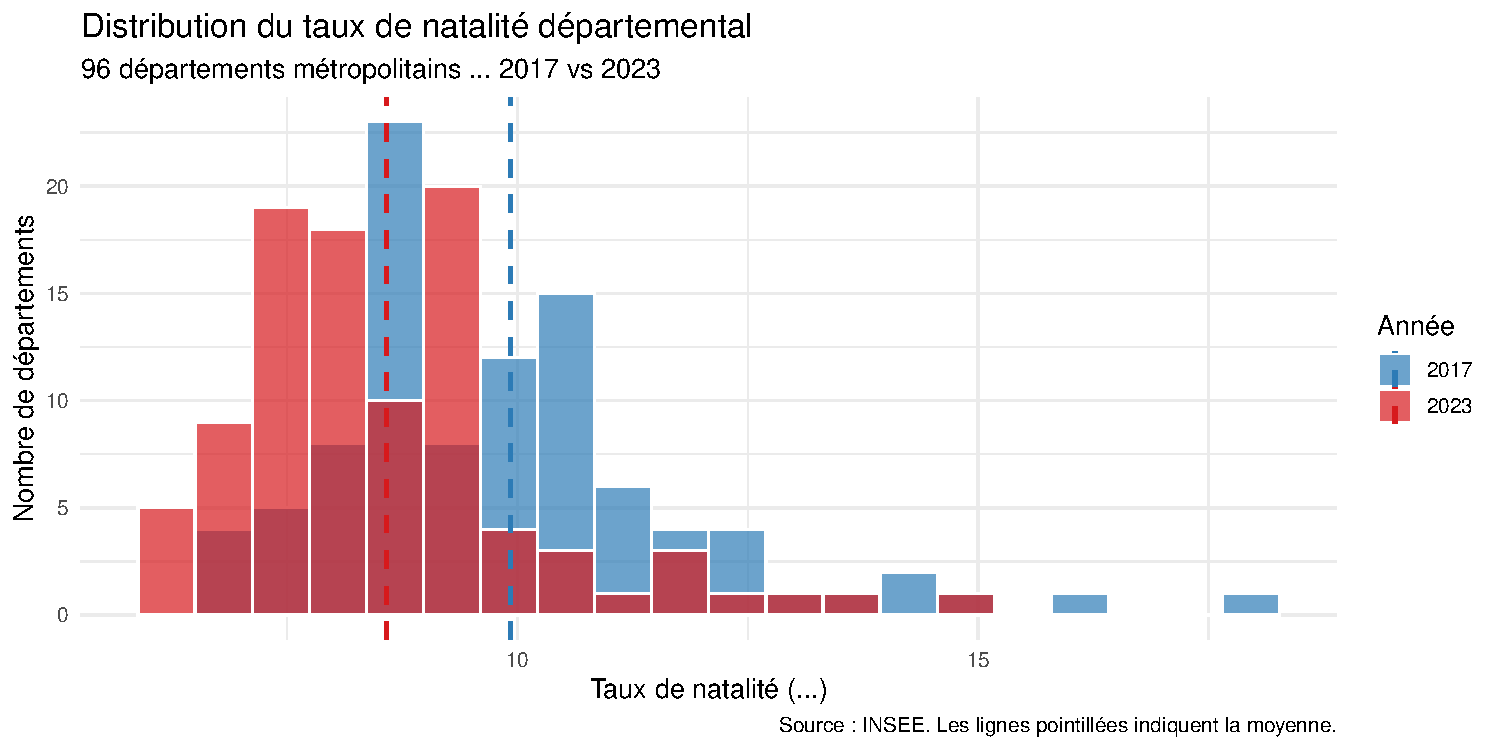
\includegraphics[keepaspectratio]{homework-6_files/figure-pdf/distrib-natalite-1.pdf}}

\textbf{Lecture.} La distribution est asymétrique à droite dans les deux
années : la majorité des départements se concentre entre 8 et 12 ‰, mais
une queue droite tirée vers le haut est visible. Ce phénomène s'explique
par quelques départements urbains à forte population immigrée, au
premier rang desquels la Seine-Saint-Denis (17,8 ‰ en 2017, 15,5 ‰ en
2023). L'ensemble de la distribution se déplace vers la gauche entre les
deux années --- illustrant que la baisse de natalité est un phénomène
généralisé à tous les départements et non concentré sur quelques
territoires. L'écart-type se réduit légèrement (de 1,97 à 1,74 ‰), signe
d'une légère convergence.

\begin{center}\rule{0.5\linewidth}{0.5pt}\end{center}

\subsection{Carte du taux de natalité en
2023}\label{carte-du-taux-de-natalituxe9-en-2023}

\texttt{\{r\ libs-carto\ ,\ message=FALSE,\ warning=FALSE\}\ library(leaflet)\ library(sf)\ library(htmlwidgets)}

```\{r carte-prep \} \# Chargement du shapefile et correction du cas
Lyon (69D / 69M → 69) dpt \textless-
sf::st\_read(``departements-20180101-shp'', quiet = TRUE)

dpt{[}dpt\(code_insee %in% c("69D", "69M"), "code_insee"] <- "69"
dpt[dpt\)nom \%in\% c(``Rhône'', ``Métropole de Lyon''), ``nom''{]}
\textless- ``Rhône'' dpt \textless- dpt \textbar\textgreater{}
select(code\_insee, nom, geometry) dpt \textless- dplyr::rename(dpt,
Code.de.département = code\_insee)

\section{Fusion des deux polygones Rhône en un
seul}\label{fusion-des-deux-polygones-rhuxf4ne-en-un-seul}

y \textless- sf::st\_union(dpt{[}dpt\$Code.de.département == ``69'',
{]}) dpt \textless- dpt \textbar\textgreater{}
dplyr::add\_row(Code.de.département = ``69'', nom = ``Rhône'', geometry
= y) \textbar\textgreater{} dplyr::slice(-c(64, 65))

\section{Jointure avec les données
2023}\label{jointure-avec-les-donnuxe9es-2023}

dpt \textless- dpt \textbar\textgreater{} left\_join(final23, by =
``Code.de.département'')

\begin{verbatim}

```{r carte-natalite
, fig.cap="Taux de natalité départemental en 2023 (‰)"}
# Palette par classes discrètes pour une lecture claire
pal_nat <- colorBin(
  palette  = "YlOrRd",
  domain   = dpt$taux_natalite_2023,
  bins     = c(5, 7, 8, 9, 10, 11, 13, 16),
  na.color = "#d9d9d9"
)

leaflet(data = dpt) |>
  addProviderTiles(providers$CartoDB.Positron) |>
  setView(lng = 2.2137, lat = 46.2276, zoom = 6) |>
  addPolygons(
    fillColor      = ~pal_nat(taux_natalite_2023),
    fillOpacity    = 0.85,
    color          = "#555555",
    weight         = 0.8,
    label          = ~nom,
    popup          = ~paste0("<b>", nom, "</b><br>Taux de natalité 2023 : ",
                             round(taux_natalite_2023, 2), " ‰"),
    highlightOptions = highlightOptions(weight = 2, color = "#000",
                                        fillOpacity = 0.95, bringToFront = TRUE)
  ) |>
  addLegend(pal = pal_nat, values = ~taux_natalite_2023,
            title = "Taux de natalité (‰)", position = "bottomright",
            opacity = 0.85) |>
  addScaleBar(position = "bottomleft",
              options  = scaleBarOptions(imperial = FALSE))
\end{verbatim}

\textbf{Lecture.} La carte révèle une \textbf{géographie de la natalité
très contrastée} en 2023. Les taux les plus élevés se concentrent dans
les grandes métropoles et leurs couronnes (Seine-Saint-Denis, Guyane
exclue de l'échantillon, Hérault, Loire-Atlantique), ainsi que dans
certains départements du littoral atlantique réputés dynamiques
démographiquement. À l'inverse, les départements du Massif central, de
la Bretagne intérieure et du grand quart nord-est affichent les valeurs
les plus faibles, témoignant du vieillissement structurel de ces
territoires. Cette hétérogénéité spatiale justifie l'approche en double
différence retenue dans l'estimation : elle permet de contrôler les
effets fixes départementaux et d'isoler la variation dans le temps.

\begin{center}\rule{0.5\linewidth}{0.5pt}\end{center}

\subsection{Carte du taux de couverture petite enfance en
2023}\label{carte-du-taux-de-couverture-petite-enfance-en-2023}

```\{r carte-couverture \} pal\_couv \textless- colorBin( palette =
``Greens'', domain = dpt\$Taux.de.couv.global, bins = c(35, 50, 57, 63,
70, 77, 86), na.color = ``\#d9d9d9'' )

leaflet(data = dpt) \textbar\textgreater{}
addProviderTiles(providers\$CartoDB.Positron) \textbar\textgreater{}
setView(lng = 2.2137, lat = 46.2276, zoom = 6) \textbar\textgreater{}
addPolygons( fillColor = \textasciitilde pal\_couv(Taux.de.couv.global),
fillOpacity = 0.85, color = ``\#555555'', weight = 0.8, label =
\textasciitilde nom, popup = \textasciitilde paste0(``'', nom, ``Taux de
couverture global 2023 :'', round(Taux.de.couv.global, 1), '' \%``),
highlightOptions = highlightOptions(weight = 2, color =''\#000'',
fillOpacity = 0.95, bringToFront = TRUE) ) \textbar\textgreater{}
addLegend(pal = pal\_couv, values = \textasciitilde Taux.de.couv.global,
title = ``Taux de couverture global (\%)'', position = ``bottomright'',
opacity = 0.85) \textbar\textgreater{} addScaleBar(position =
``bottomleft'', options = scaleBarOptions(imperial = FALSE))

\begin{verbatim}

**Lecture.** La couverture petite enfance présente une géographie sensiblement 
différente de celle de la natalité. Les départements les mieux dotés en 2023 
sont essentiellement ruraux et de l'Ouest (Vendée, Mayenne, Maine-et-Loire, 
Haute-Loire), où l'accueil individuel par assistantes maternelles est 
historiquement très développé. À l'inverse, la Corse-du-Sud (38,9 %) et la 
Seine-Saint-Denis (40,9 %) affichent les taux les plus faibles — paradoxe 
apparent pour ce dernier département qui combine le taux de natalité le plus 
élevé de France et l'une des couvertures les plus basses, illustrant 
précisément la tension entre demande non satisfaite et offre insuffisante que 
cette étude cherche à analyser.

---

## Distribution du taux de couverture global


::: {.cell}

```{.r .cell-code}
df_couv <- bind_rows(
  final17 |> select(Taux.de.couv.global) |> mutate(Année = "2017"),
  final23 |> select(Taux.de.couv.global) |> mutate(Année = "2023")
)

ggplot(df_couv, aes(x = Taux.de.couv.global, fill = Année)) +
  geom_histogram(bins = 20, alpha = 0.7, position = "identity", color = "white") +
  geom_vline(
    data = df_couv |> group_by(Année) |> summarise(m = mean(Taux.de.couv.global)),
    aes(xintercept = m, color = Année), linetype = "dashed", linewidth = 1
  ) +
  scale_fill_manual(values  = c("2017" = "#1a9641", "2023" = "#fdae61")) +
  scale_color_manual(values = c("2017" = "#1a9641", "2023" = "#fdae61")) +
  theme_minimal(base_size = 13) +
  labs(
    title    = "Distribution du taux de couverture global de la petite enfance",
    subtitle = "96 départements métropolitains — 2017 vs 2023",
    x        = "Taux de couverture global (%)",
    y        = "Nombre de départements",
    caption  = "Source : CNAF. Les lignes pointillées indiquent la moyenne."
  )
\end{verbatim}

\pandocbounded{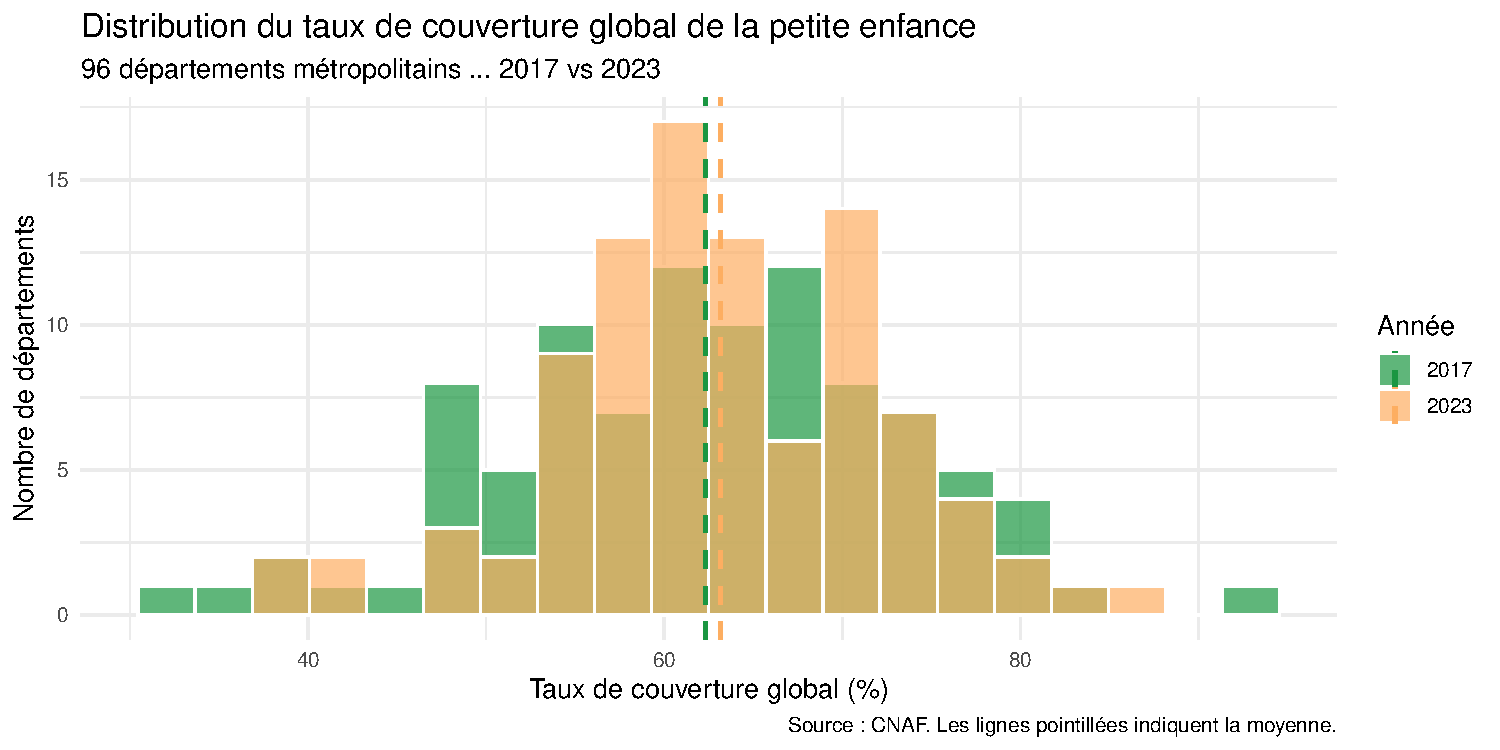
\includegraphics[keepaspectratio]{homework-6_files/figure-pdf/distrib-couverture-1.pdf}}

:::

\textbf{Lecture.} La distribution du taux de couverture global est
approximativement normale, centrée autour de 62--63 \%. Entre 2017 et
2023, la moyenne progresse légèrement (+0,87 point) et l'écart-type se
réduit notablement (11,25 → 9,45), témoignant d'un \textbf{rattrapage
des départements les moins bien dotés}. En 2017, la Haute-Loire
affichait le taux le plus élevé (92,6 \%) tandis que la
Seine-Saint-Denis le plus faible (31,7 \%) ; en 2023, l'amplitude se
resserre, la Vendée prenant la tête (85,7 \%) et la Corse-du-Sud le bas
du classement (38,9 \%). La convergence observée est compatible avec les
politiques de développement de l'accueil menées par la CNAF sur cette
période.

\begin{center}\rule{0.5\linewidth}{0.5pt}\end{center}

\subsection{Accueil collectif versus accueil
individuel}\label{accueil-collectif-versus-accueil-individuel}

\begin{Shaded}
\begin{Highlighting}[]
\NormalTok{df\_type }\OtherTok{\textless{}{-}} \FunctionTok{bind\_rows}\NormalTok{(}
\NormalTok{  final17 }\SpecialCharTok{|\textgreater{}}
    \FunctionTok{select}\NormalTok{(département,}
           \AttributeTok{Collectif  =}\NormalTok{ Taux.de.couv.collectif,}
           \AttributeTok{Individuel =}\NormalTok{ Taux.de.couv.individuel) }\SpecialCharTok{|\textgreater{}}
    \FunctionTok{pivot\_longer}\NormalTok{(}\SpecialCharTok{{-}}\NormalTok{département, }\AttributeTok{names\_to =} \StringTok{"Type"}\NormalTok{, }\AttributeTok{values\_to =} \StringTok{"taux"}\NormalTok{) }\SpecialCharTok{|\textgreater{}}
    \FunctionTok{mutate}\NormalTok{(Année }\OtherTok{=} \StringTok{"2017"}\NormalTok{),}
\NormalTok{  final23 }\SpecialCharTok{|\textgreater{}}
    \FunctionTok{select}\NormalTok{(département,}
           \AttributeTok{Collectif  =}\NormalTok{ Taux.de.couv.collectif,}
           \AttributeTok{Individuel =}\NormalTok{ Taux.de.couv.individuel) }\SpecialCharTok{|\textgreater{}}
    \FunctionTok{pivot\_longer}\NormalTok{(}\SpecialCharTok{{-}}\NormalTok{département, }\AttributeTok{names\_to =} \StringTok{"Type"}\NormalTok{, }\AttributeTok{values\_to =} \StringTok{"taux"}\NormalTok{) }\SpecialCharTok{|\textgreater{}}
    \FunctionTok{mutate}\NormalTok{(Année }\OtherTok{=} \StringTok{"2023"}\NormalTok{)}
\NormalTok{)}

\NormalTok{df\_type }\SpecialCharTok{|\textgreater{}}
  \FunctionTok{group\_by}\NormalTok{(Année, Type) }\SpecialCharTok{|\textgreater{}}
  \FunctionTok{summarise}\NormalTok{(}\AttributeTok{moy =} \FunctionTok{mean}\NormalTok{(taux, }\AttributeTok{na.rm =} \ConstantTok{TRUE}\NormalTok{), }\AttributeTok{.groups =} \StringTok{"drop"}\NormalTok{) }\SpecialCharTok{|\textgreater{}}
  \FunctionTok{ggplot}\NormalTok{(}\FunctionTok{aes}\NormalTok{(}\AttributeTok{x =}\NormalTok{ Année, }\AttributeTok{y =}\NormalTok{ moy, }\AttributeTok{fill =}\NormalTok{ Type)) }\SpecialCharTok{+}
  \FunctionTok{geom\_col}\NormalTok{(}\AttributeTok{position =} \StringTok{"dodge"}\NormalTok{, }\AttributeTok{width =} \FloatTok{0.5}\NormalTok{) }\SpecialCharTok{+}
  \FunctionTok{geom\_text}\NormalTok{(}\FunctionTok{aes}\NormalTok{(}\AttributeTok{label =} \FunctionTok{round}\NormalTok{(moy, }\DecValTok{1}\NormalTok{)), }\AttributeTok{position =} \FunctionTok{position\_dodge}\NormalTok{(}\AttributeTok{width =} \FloatTok{0.5}\NormalTok{),}
            \AttributeTok{vjust =} \SpecialCharTok{{-}}\FloatTok{0.4}\NormalTok{, }\AttributeTok{size =} \DecValTok{4}\NormalTok{) }\SpecialCharTok{+}
  \FunctionTok{scale\_fill\_manual}\NormalTok{(}\AttributeTok{values =} \FunctionTok{c}\NormalTok{(}\StringTok{"Collectif"} \OtherTok{=} \StringTok{"\#2c7bb6"}\NormalTok{, }\StringTok{"Individuel"} \OtherTok{=} \StringTok{"\#d7191c"}\NormalTok{)) }\SpecialCharTok{+}
  \FunctionTok{theme\_minimal}\NormalTok{(}\AttributeTok{base\_size =} \DecValTok{13}\NormalTok{) }\SpecialCharTok{+}
  \FunctionTok{labs}\NormalTok{(}
    \AttributeTok{title    =} \StringTok{"Taux de couverture moyen par type d\textquotesingle{}accueil"}\NormalTok{,}
    \AttributeTok{subtitle =} \StringTok{"Moyenne sur 96 départements métropolitains"}\NormalTok{,}
    \AttributeTok{x        =} \ConstantTok{NULL}\NormalTok{, }\AttributeTok{y =} \StringTok{"Taux de couverture moyen (\%)"}\NormalTok{,}
    \AttributeTok{caption  =} \StringTok{"Source : CNAF."}
\NormalTok{  )}
\end{Highlighting}
\end{Shaded}

\pandocbounded{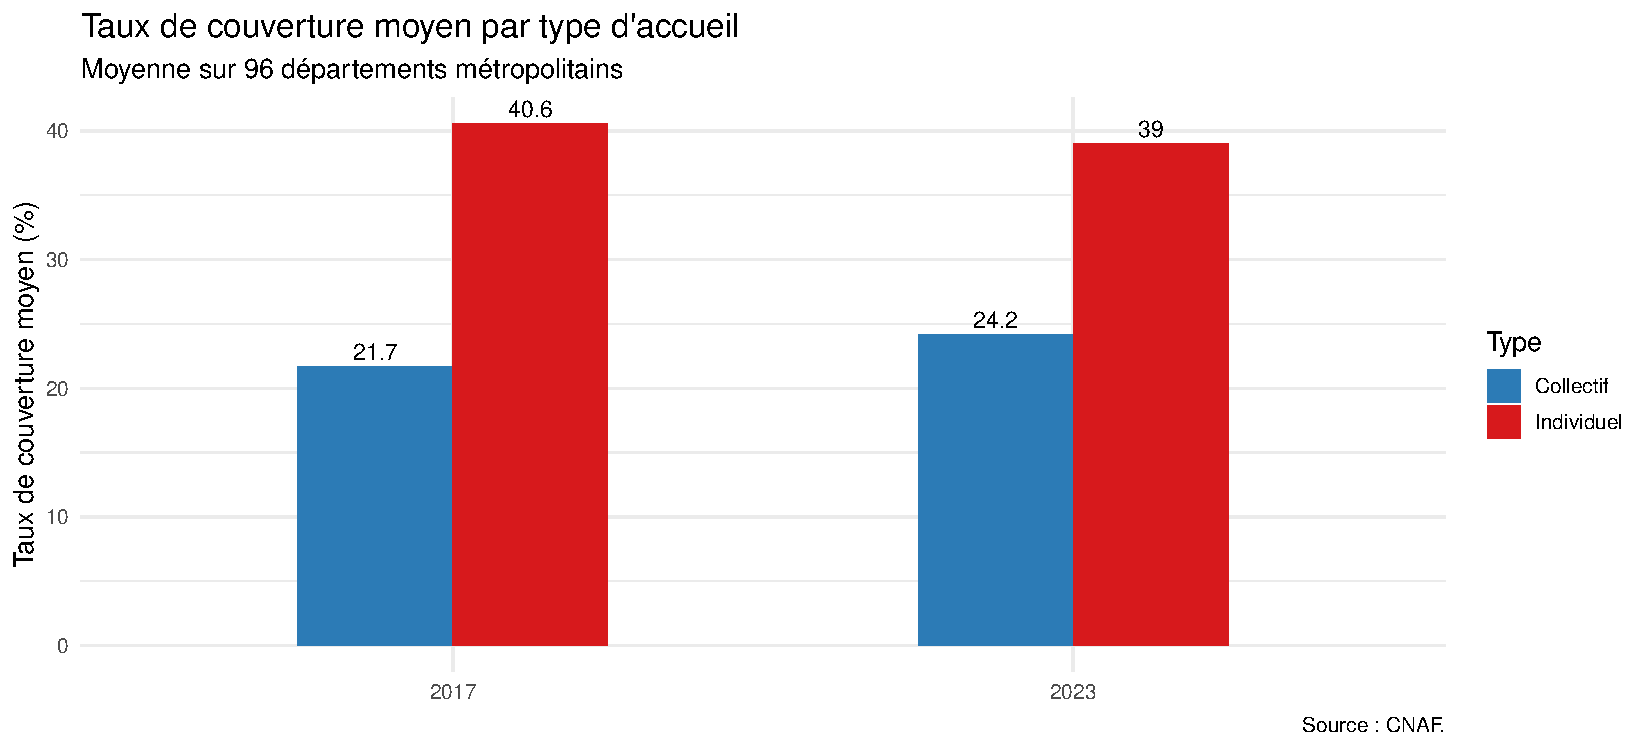
\includegraphics[keepaspectratio]{homework-6_files/figure-pdf/graph-collectif-individuel-1.pdf}}

\textbf{Lecture.} En 2017, l'accueil individuel (assistantes maternelles
+ salariées à domicile) représente en moyenne \textbf{40,6 \%} de
couverture contre \textbf{21,7 \%} pour l'accueil collectif, soit une
part de 65 \% pour l'individuel dans la couverture totale. En 2023, ce
rapport évolue légèrement en faveur du collectif (24,2 \% vs 39,0 \%),
reflétant les efforts d'investissement dans les structures EAJE sur
cette période. La \textbf{prédominance de l'accueil individuel} est un
trait structurel du système français qui distingue la France de ses
voisins nordiques, où les crèches collectives sont plus développées.
Cette distinction sera exploitée dans l'estimation pour tester si
l'effet sur la natalité diffère selon le mode d'accueil.

\begin{center}\rule{0.5\linewidth}{0.5pt}\end{center}

\subsection{Corrélation préliminaire : natalité et
couverture}\label{corruxe9lation-pruxe9liminaire-natalituxe9-et-couverture}

\begin{Shaded}
\begin{Highlighting}[]
\FunctionTok{ggplot}\NormalTok{(final23, }\FunctionTok{aes}\NormalTok{(}\AttributeTok{x =}\NormalTok{ Taux.de.couv.global, }\AttributeTok{y =}\NormalTok{ taux\_natalite\_2023)) }\SpecialCharTok{+}
  \FunctionTok{geom\_point}\NormalTok{(}\AttributeTok{alpha =} \FloatTok{0.7}\NormalTok{, }\AttributeTok{size =} \FloatTok{2.5}\NormalTok{, }\AttributeTok{color =} \StringTok{"\#2c7bb6"}\NormalTok{) }\SpecialCharTok{+}
  \FunctionTok{geom\_smooth}\NormalTok{(}\AttributeTok{method =} \StringTok{"lm"}\NormalTok{, }\AttributeTok{se =} \ConstantTok{TRUE}\NormalTok{, }\AttributeTok{color =} \StringTok{"\#d7191c"}\NormalTok{, }\AttributeTok{linewidth =} \DecValTok{1}\NormalTok{) }\SpecialCharTok{+}
  \FunctionTok{geom\_text\_repel}\NormalTok{(}
    \AttributeTok{data =}\NormalTok{ final23 }\SpecialCharTok{|\textgreater{}}
      \FunctionTok{filter}\NormalTok{(taux\_natalite\_2023 }\SpecialCharTok{\textgreater{}} \DecValTok{12} \SpecialCharTok{|}\NormalTok{ taux\_natalite\_2023 }\SpecialCharTok{\textless{}} \DecValTok{7} \SpecialCharTok{|}
\NormalTok{             Taux.de.couv.global }\SpecialCharTok{\textgreater{}} \DecValTok{80} \SpecialCharTok{|}\NormalTok{ Taux.de.couv.global }\SpecialCharTok{\textless{}} \DecValTok{45}\NormalTok{),}
    \FunctionTok{aes}\NormalTok{(}\AttributeTok{label =} \FunctionTok{gsub}\NormalTok{(}\StringTok{"\^{}[0{-}9A{-}Z]+{-}"}\NormalTok{, }\StringTok{""}\NormalTok{, département)),}
    \AttributeTok{size =} \DecValTok{3}\NormalTok{, }\AttributeTok{max.overlaps =} \DecValTok{12}
\NormalTok{  ) }\SpecialCharTok{+}
  \FunctionTok{theme\_minimal}\NormalTok{(}\AttributeTok{base\_size =} \DecValTok{13}\NormalTok{) }\SpecialCharTok{+}
  \FunctionTok{labs}\NormalTok{(}
    \AttributeTok{title    =} \StringTok{"Taux de natalité et couverture petite enfance en 2023"}\NormalTok{,}
    \AttributeTok{subtitle =} \FunctionTok{paste0}\NormalTok{(}\StringTok{"Corrélation de Pearson = "}\NormalTok{,}
                      \FunctionTok{round}\NormalTok{(}\FunctionTok{cor}\NormalTok{(final23}\SpecialCharTok{$}\NormalTok{taux\_natalite\_2023,}
\NormalTok{                                final23}\SpecialCharTok{$}\NormalTok{Taux.de.couv.global,}
                                \AttributeTok{use =} \StringTok{"complete.obs"}\NormalTok{), }\DecValTok{3}\NormalTok{)),}
    \AttributeTok{x        =} \StringTok{"Taux de couverture global (\%)"}\NormalTok{,}
    \AttributeTok{y        =} \StringTok{"Taux de natalité (‰)"}\NormalTok{,}
    \AttributeTok{caption  =} \StringTok{"Source : CNAF / INSEE. 96 départements métropolitains."}
\NormalTok{  )}
\end{Highlighting}
\end{Shaded}

\pandocbounded{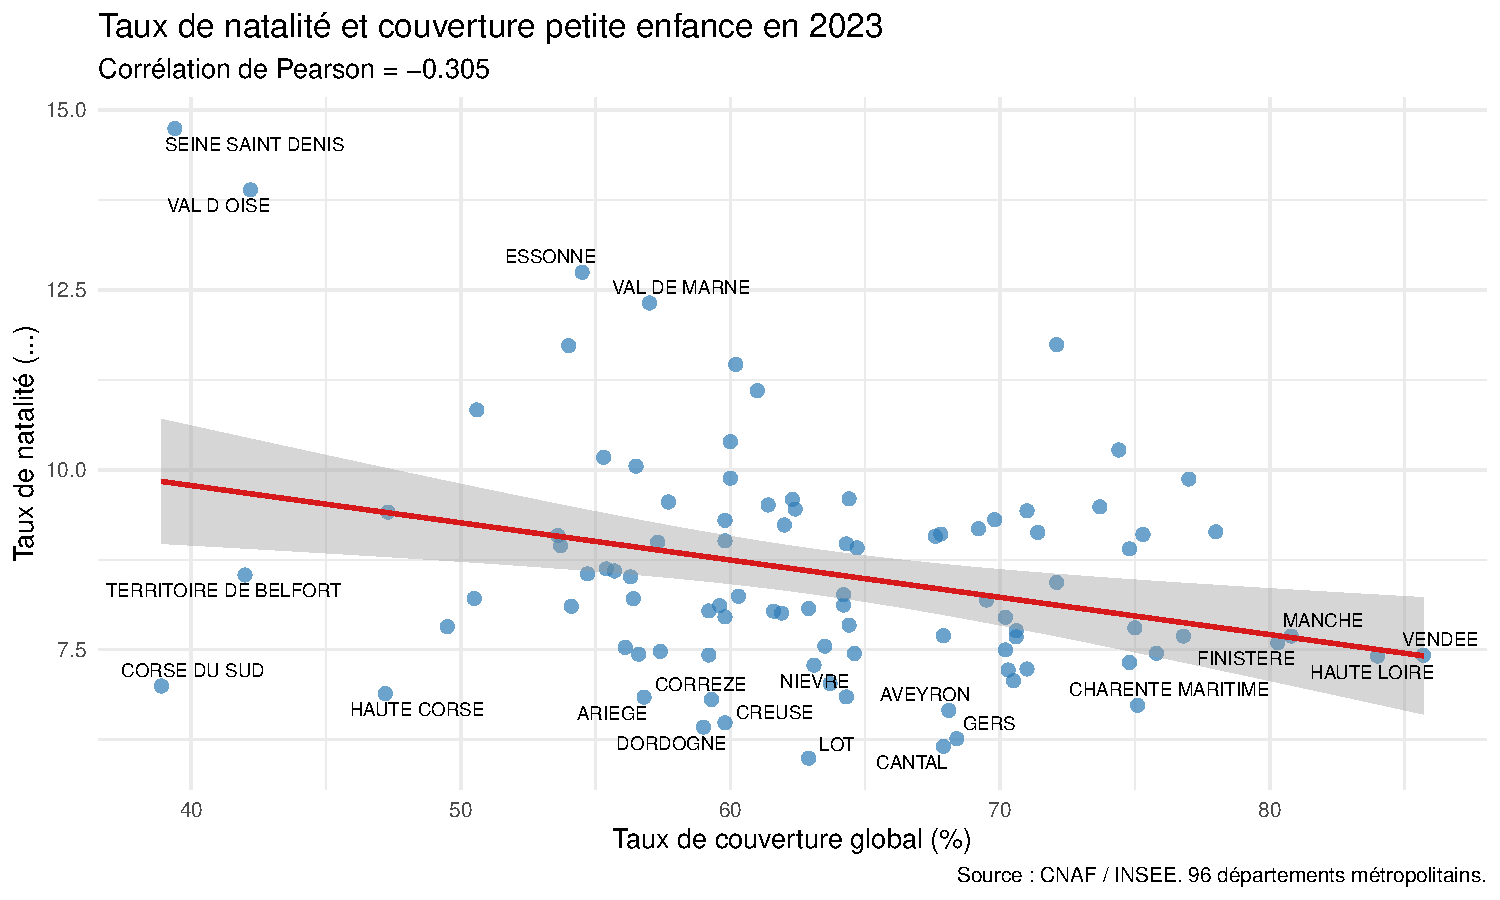
\includegraphics[keepaspectratio]{homework-6_files/figure-pdf/scatterplot-principal-1.pdf}}

\textbf{Lecture.} La corrélation brute entre taux de couverture global
et taux de natalité est \textbf{négative} (r = −0,316 en 2023, r =
−0,400 en 2017). Ce résultat, contre-intuitif au regard des
recommandations politiques, s'explique par deux mécanismes de biais :
d'une part une \textbf{causalité inverse} (les politiques publiques de
garde se développent en réponse à une demande elle-même liée à la
démographie locale), d'autre part la présence de \textbf{variables
confondantes} --- notamment la structure économique du territoire.
L'indice d'emploi est d'ailleurs positivement corrélé à la natalité (r =
0,34 en 2017), ce qui indique que les départements dynamiques
économiquement sont à la fois plus natalistes et plus dotés en emplois
--- et donc potentiellement en modes de garde. La corrélation brute ne
reflète donc pas l'effet causal recherché. C'est précisément pour
corriger ces biais que la stratégie en double différence est mobilisée
dans la section suivante.

\begin{center}\rule{0.5\linewidth}{0.5pt}\end{center}

\emph{Suite dans le prochain chat : Partie 4 --- Stratégie
d'identification et estimation (double différence)}




\end{document}
